\documentclass{article}

% if you need to pass options to natbib, use, e.g.:
%     \PassOptionsToPackage{numbers, compress}{natbib}
% before loading neurips_2026

% The authors should use one of these tracks.
% Before accepting by the NeurIPS conference, select one of the options below.
% 0. "default" for submission
\usepackage{neurips_2026}
% the "default" option is equal to the "main" option, which is used for the Main Track with double-blind reviewing.
% 1. "main" option is used for the Main Track
%  \usepackage[main]{neurips_2026}
% 2. "position" option is used for the Position Paper Track
%  \usepackage[position]{neurips_2026}
% 3. "eandd" option is used for the Evaluations & Datasets Track
 % \usepackage[eandd]{neurips_2026}
% 4. "creativeai" option is used for the Creative AI Track
%  \usepackage[creativeai]{neurips_2026}
% 5. "sglblindworkshop" option is used for the Workshop with single-blind reviewing
 % \usepackage[sglblindworkshop]{neurips_2026}
% 6. "dblblindworkshop" option is used for the Workshop with double-blind reviewing
%  \usepackage[dblblindworkshop]{neurips_2026}

% After being accepted, the authors should add "final" behind the track to compile a camera-ready version.
% 1. Main Track
 % \usepackage[main, final]{neurips_2026}
% 2. Position Paper Track
%  \usepackage[position, final]{neurips_2026}
% 3. Evaluations & Datasets Track
 % \usepackage[eandd, final]{neurips_2026}
% 4. Creative AI Track
%  \usepackage[creativeai, final]{neurips_2026}
% 5. Workshop with single-blind reviewing
%  \usepackage[sglblindworkshop, final]{neurips_2026}
% 6. Workshop with double-blind reviewing
%  \usepackage[dblblindworkshop, final]{neurips_2026}
% Note. For the workshop paper template, both \title{} and \workshoptitle{} are required, with the former indicating the paper title shown in the title and the latter indicating the workshop title displayed in the footnote.
% For workshops (5., 6.), the authors should add the name of the workshop, "\workshoptitle" command is used to set the workshop title.
% \workshoptitle{WORKSHOP TITLE}

% "preprint" option is used for arXiv or other preprint submissions
 % \usepackage[preprint]{neurips_2026}

% to avoid loading the natbib package, add option nonatbib:
%    \usepackage[nonatbib]{neurips_2026}

\usepackage[utf8]{inputenc} % allow utf-8 input
\usepackage[T1]{fontenc}    % use 8-bit T1 fonts
\usepackage{hyperref}       % hyperlinks
\usepackage{url}            % simple URL typesetting
\usepackage{booktabs}       % professional-quality tables
\usepackage{amsfonts}       % blackboard math symbols
\usepackage{nicefrac}       % compact symbols for 1/2, etc.
\usepackage{microtype}      % microtypography
\usepackage{xcolor}         % colors
\usepackage{caption}
\usepackage{graphicx}
\usepackage{amsmath}
\usepackage{multirow}
\usepackage{amsmath, amsfonts, amssymb, amsthm}
\usepackage{booktabs}
\usepackage{algorithm}
\usepackage{algorithmic}
\usepackage{svg}

\newtheorem{theorem}{Theorem}
\newtheorem{proposition}{Proposition}
\newtheorem{lemma}{Lemma}

\title{Uncertainty-Aware Offline Data-Driven Multi-Objective Optimization}

\author{%
  David S.~Hippocampus\thanks{Use footnote for providing further information
    about author (webpage, alternative address)---\emph{not} for acknowledging
    funding agencies.} \\
  Department of Computer Science\\
  Cranberry-Lemon University\\
  Pittsburgh, PA 15213 \\
  \texttt{hippo@cs.cranberry-lemon.edu} \\
  % examples of more authors
  % \And
  % Coauthor \\
  % Affiliation \\
  % Address \\
  % \texttt{email} \\
  % \AND
  % Coauthor \\
  % Affiliation \\
  % Address \\
  % \texttt{email} \\
  % \And
  % Coauthor \\
  % Affiliation \\
  % Address \\
  % \texttt{email} \\
  % \And
  % Coauthor \\
  % Affiliation \\
  % Address \\
  % \texttt{email} \\
}


\begin{document}


\maketitle


\begin{abstract}
In offline data-driven multi-objective optimization (MOO), optimization is performed using surrogate models trained only on an offline dataset. These surrogate models contain inherent errors and uncertainty. This epistemic uncertainty can lead to incorrect dominance judgments, thereby misleading the search process. Existing methods mitigate this issue by incorporating uncertainty estimates from Gaussian Process Regression (GPR) to correct dominance judgments; however, they are restricted to GPR, and their optimization strategies cannot be scaled to other uncertainty quantification methods. In addition, GPR-based surrogates suffer from high computational cost. We propose a simple yet effective dual-ranking strategy that flexibly leverages both predictive results and uncertainty estimates from different surrogate models. By performing non-dominated sorting on candidate solutions using both surrogate-based fitness values and uncertainty-aware fitness values, the proposed method prioritizes candidate solutions that are simultaneously high-quality and reliable. Through extensive experimental evaluations, we demonstrate the effectiveness and robustness of the proposed dual-ranking strategy working with different surrogates. Our dual-ranking framework offers more robust solutions for data-limited, real-world applications. The source code is available at https://anonymous.4open.science/r/Nips-2026-hhh/.
\end{abstract}



\section{Introduction}
% 1. Big background
In real-world applications, many Multi-objective Optimization Problems (MOPs), namely, those involving multiple objectives to be optimized, lack analytical functions or simulation models that allow for direct evaluation~\cite{ddeo_rvea}. Consequently, data-driven Multi-Objective Evolutionary Algorithms (MOEAs) have gained prominence by combining learning-based techniques with robust evolutionary search capabilities. These methods have proven effective in various applications, including trauma systems, airfoil design, energy systems, and smart building optimization \cite{ddeo_1,ddeo_2,ddeo_ibea,building_opt2}.

% 2. General challenges in DDEA
Despite their success, offline data-driven MOEAs face a critical challenge. Objective values are solely estimated via surrogates (\emph{i.e.}, data-driven models). Unlike surrogate-assisted optimization, no further real evaluations are available to improve the prediction accuracy. Even with a noise-free offline dataset where aleatoric uncertainty can be neglected, surrogate models still suffer from epistemic uncertainty arising from limited or biased training data, model selection, and training procedures. This approximation uncertainty can severely degrade optimization performance~\cite{ddeo_2} by misleading the search, resulting in suboptimal solutions \cite{optimizer_curse}. As shown in Figure~\ref{fig_1}, relying solely on surrogate-based evaluations $f_{\text{sur}}$ can lead to an incorrect dominance judgment, whereas incorporating uncertainty estimates can correct it in such cases.

\begin{figure}[htbp]
    \centering
    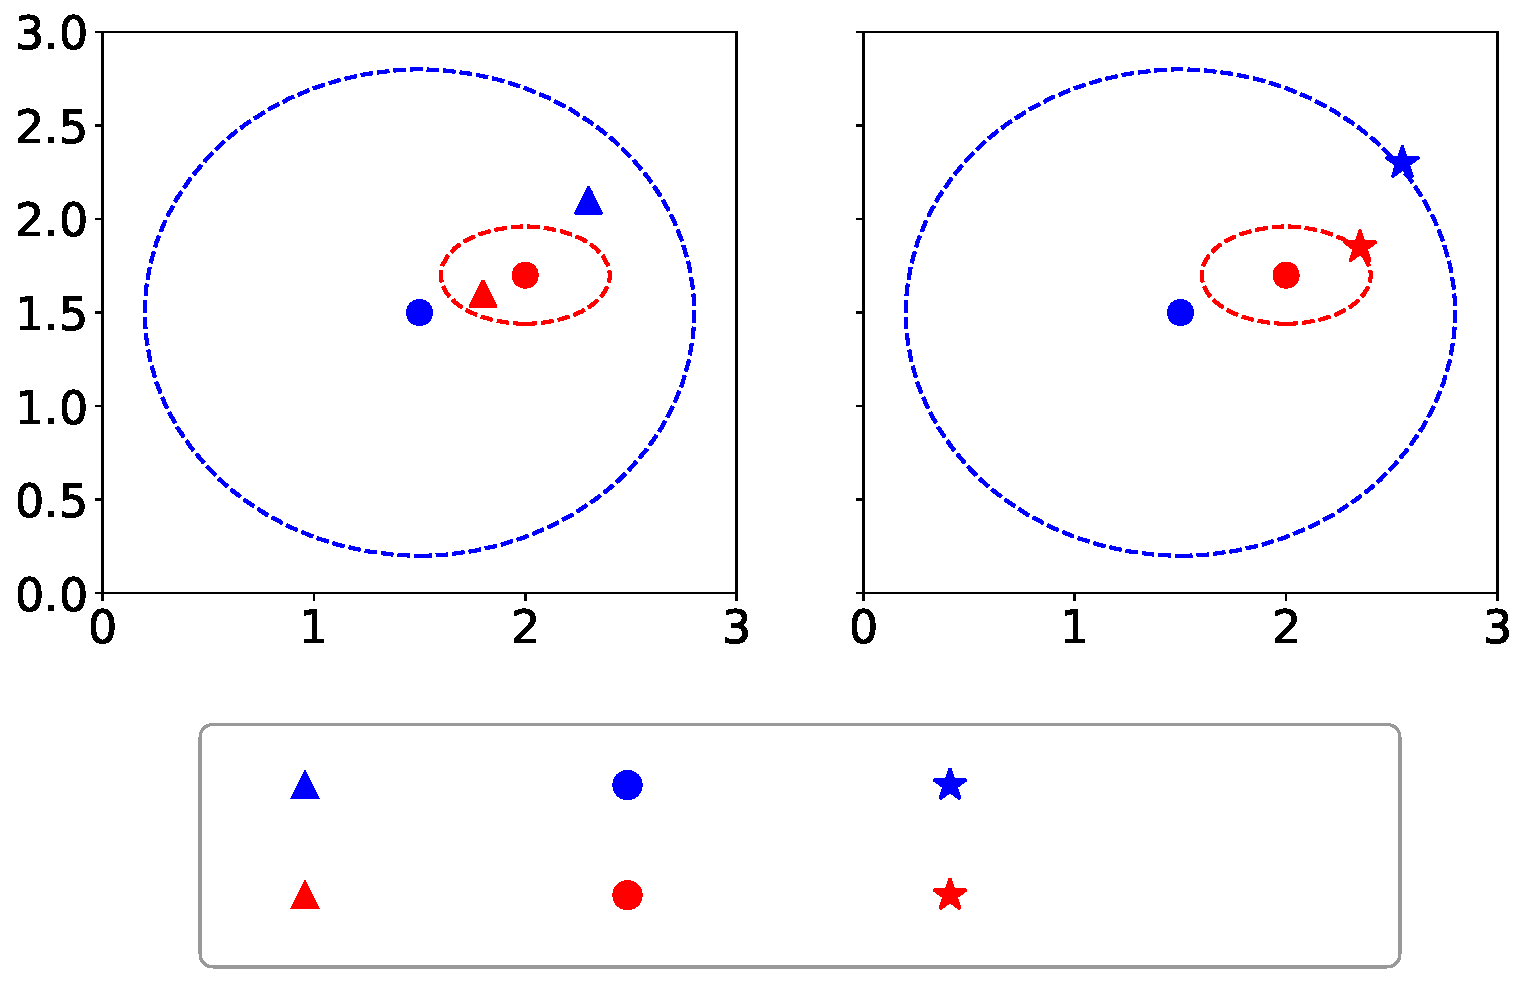
\includegraphics[width=0.7\linewidth]
    {fig_1.pdf}
    \put(-200,57){$f_1$}
    \put(-65,57){$f_1$}
    \put(-285,120){$f_2$}
    \put(-217,32){$f_\text{real}(\boldsymbol{A})$}
    \put(-217,12){$f_\text{real}(\boldsymbol{B})$}
    \put(-157,32){$f_\text{sur}(\boldsymbol{A})$}
    \put(-157,12){$f_\text{sur}(\boldsymbol{B})$}
    \put(-97,32){$f_\text{UA-sur}(\boldsymbol{A})$}
    \put(-97,12){$f_\text{UA-sur}(\boldsymbol{B})$}
\caption{An example of misleading dominance ranking in a minimization problem induced by surrogate-based evaluations and its correction via uncertainty-aware fitness values. The dashed circle denotes the predictive uncertainty interval centered at the surrogate-predicted objective values. Left: Relying solely on surrogate-based evaluations ($f_\text{sur}(\boldsymbol{A})$ and $f_\text{sur}(\boldsymbol{B})$) leads to an incorrect dominance judgment, $\boldsymbol{A} \prec \boldsymbol{B}$, which contradicts the dominance judgment under real evaluations, $\boldsymbol{B} \prec \boldsymbol{A}$. Right: Incorporating uncertainty estimates through uncertainty-aware surrogate-based evaluations ($f_\text{UA-sur}(\boldsymbol{A})$ and $f_\text{UA-sur}(\boldsymbol{B})$) may result in $\boldsymbol{B} \prec \boldsymbol{A}$.}
\label{fig_1}
\end{figure}

% 3. Existing methods (ensemble) and issues
To mitigate this issue, existing approaches include reducing approximation uncertainty through ensemble methods, and quantifying the uncertainty for incorporation into the optimization process. For the former, various ensemble methods have been proposed, such as selective surrogate ensembles~\cite{ddeo_2}, perturbation-based ensemble surrogates~\cite{ddeo_3} and ensemble surrogates with tri-training~\cite{ddeo_4}. However, these methods do not explicitly incorporate uncertainty information during optimization. Consequently, accumulated prediction errors can largely compromise the search process, potentially leading to suboptimal outcomes~\cite{ddeo_ibea}.

% 4. Existing methods (uncertainty information)
For the second approach, Kriging, also known as Gaussian Process Regression (GPR), is commonly adopted as the surrogate model due to its ability to provide uncertainty estimates~\cite{gpr}. Several methods leverage it, such as IBEA-MS~\cite{ddeo_ibea}, Prob-RVEA and Prob-MOEA/D~\cite{ddeo_rvea}. In addition, TGPR-MO~\cite{ddeo-TGPR} combines regression trees with GPR to handle large datasets. DDMOEA/GAN~\cite{ddea_gan} utilizes discriminator and generator mechanisms of a generative adversarial network (GAN) for trust-aware evaluation and data augmentation, respectively.

% 5. Issues and our methods 
In this vein, existing studies often rely on the predictive mean and standard deviation from GPR models to adjust model selection or perform Monte Carlo sampling. However, these methods are typically restricted to GPR and may suffer from high computational cost when the surrogate is trained on a large dataset. We consider a different perspective that directly incorporates uncertainty estimates into the fitness assignment procedure of a MOEA. Our contributions are summarized as follows:

\begin{itemize}
  \item \textbf{Dual-Ranking Strategy.}
  To prioritize solutions that are both high-quality and reliable, while avoiding misleading rankings, we propose a dual-ranking strategy that considers the non-dominated front using both the surrogate-based function $f_{\text{sur}}$ and the uncertainty-aware function $f_{\text{UA-sur}}$. The proposed strategy can be flexibly integrated with different surrogate models.
  
  \item \textbf{Auto-$\alpha$ Selection Algorithm.}
  To align the uncertainty estimates from GPR with the quantile-based function, we design an auto-$\alpha$ selection algorithm to determine the hyperparameter $\alpha$ based on the target coverage $\tau$.
  
  \item \textbf{Extensive Evaluation.}
  We integrate the proposed dual-ranking strategy with different surrogate models and conduct extensive experiments, as well as a real-world case study, to demonstrate its effectiveness and robustness under different settings.
\end{itemize}

\section{Preliminaries}
\subsection{Multi-Objective Optimization}
The MOPs are considered in the following form:
\begin{align}\label{eq:mops}
\text{minimize }& \boldsymbol{f}(\boldsymbol{x}) = \left(f_1(\boldsymbol{x}), f_2(\boldsymbol{x}), \ldots, f_K(\boldsymbol{x})\right) \nonumber \\
\text{subject to }& \boldsymbol{x} \in S,
\end{align}
where $\boldsymbol{x}$ is the decision vector, $K \geq 2$ is the total number of objectives, and $S$ is the feasible region in the decision space. A solution $\boldsymbol{x}_{1} \in S$ dominates another solution $\boldsymbol{x}_{2} \in S$, denoted as $\boldsymbol{x}_{1} \prec \boldsymbol{x}_{2}$, if $f_k(\boldsymbol{x}_{1}) \leq f_k(\boldsymbol{x}_{2})$ for all $k = 1,\ldots,K$ and $f_k(\boldsymbol{x}_{1}) < f_k(\boldsymbol{x}_{2})$ for at least one $k = 1,\ldots,K$. The set of solutions that cannot be dominated by any other feasible solution is the Pareto Set (PS), and the set of their objective values is the Pareto Front (PF).

\subsection{Offline Data-Driven vs. Surrogate-Assisted Multi-Objective Optimization}
In offline data-driven Multi-Objective Optimization (MOO), there is no explicit mathematical expression of the objective functions. Unlike surrogate-assisted optimization, which allows real evaluations to acquire new data points for improving the surrogate model during the optimization process \cite{kriging_assisted}, offline data-driven MOO works in situations where querying solutions on the fly is not accessible \cite{ddeo_ibea,ddeo_rvea}, and thus deals with a pre-collected dataset. This dataset remains unchanged during optimization. The objective functions are approximated by training surrogates on this offline dataset. %%\miqing{I have polished the above a bit, please double check it.}

\subsection{Surrogate Modeling}
The surrogate $\mathcal{M}$, trained on the offline dataset $\mathcal{D}$, aims to predict the objective values of a candidate solution $\boldsymbol{x}$. For the $k$-th objective, the surrogate prediction can be expressed as $f_{k}(\boldsymbol{x}) \approx \mathcal{M}_{k} (\boldsymbol{x})$. Existing mainstream surrogate models that can provide both predictions and uncertainty-related information include GPR \cite{gpr}, Quantile Regression (QR) \cite{quantile_regression}, Bayesian Neural Network (BNN) \cite{bnn}, and ensemble methods \cite{ddeo_2}. GPR is widely used in surrogate-assisted and offline data-driven MOO \cite{jin_gpr}, as it naturally provides predictive mean and variance. However, standard GPR suffers from high computational cost and degraded performance in high dimensions. QR does not rely on Gaussian assumptions and is useful under asymmetric or heavy-tailed distributions. BNN utilizes the strong representation ability of neural networks and is scalable to larger datasets and higher-dimensional problems, although training and inference are computationally expensive. Ensemble methods are widely used in engineering problems and commonly estimate uncertainty from multiple independently trained surrogates. In this work, we consider GPR, QR, and BNN as surrogate models.

\subsubsection{Gaussian Process Regression}
The GPR model is fully specified by a mean function $\mu(\mathbf{x})$ and a covariance (kernel) function $k(\mathbf{x}, \mathbf{x}')$
$f(\mathbf{x}) \sim \mathcal{GP}(\mu(\mathbf{x}), k(\mathbf{x}, \mathbf{x}'))$. In this work, we adopt the Gaussian kernel \cite{gaussian_kernel} 
$k(\mathbf{x}, \mathbf{x}')
=\sigma_f^2
\exp\!\left(-\tfrac{1}{2} r^2(\mathbf{x}, \mathbf{x}')\right)$,
and the Automatic Relevance Determination (ARD) Mat\'ern 5/2 kernel \cite{kernel_Matern_52}
$k_{\mathrm{M52}}(\mathbf{x}, \mathbf{x}')
=\sigma_f^2
\left(1 + \sqrt{5r^2(\mathbf{x}, \mathbf{x}')}
+ \tfrac{5}{3} r^2(\mathbf{x}, \mathbf{x}')\right)
\exp\!\left(-\sqrt{5r^2(\mathbf{x}, \mathbf{x}')}\right)$,
as the latter does not make the covariance function unrealistically smooth \cite{ddeo-TGPR}.

\subsubsection{Quantile Regression}
QR estimates the conditional quantile (\emph{e.g.} median) of a target variable. For a given quantile level $\tau \in (0, 1)$, the estimator is obtained by
$
\hat{\boldsymbol{\beta}}_\tau = \arg\min_{\boldsymbol{\beta}} \sum_{i=1}^n \rho_\tau \left( y_i - \boldsymbol{x}_i^\top \boldsymbol{\beta} \right),
$
where $\boldsymbol{\beta}$ represents the regression coefficients and the loss function $\rho_\tau(y,\hat{y})$ is the ``check function'' \cite{pinball_loss}. The simplicity and generality of this formulation makes quantile regression widely applicable across various domains \cite{conformal_quantile_regression}. We employ QR to estimate uncertainty intervals by predicting multiple conditional quantiles.

\subsubsection{Bayesian Neural Network}
BNN places probability distributions over network weights instead of point estimates, enabling the modeling of epistemic uncertainty. It approximates the posterior distribution $p(\mathbf{w} \mid \mathcal{D})$ over weights $\mathbf{w}$ using variational inference. For a given input $\boldsymbol{x}$, the predictive distribution is approximated as:
$
p(y \mid \boldsymbol{x},\mathcal{D}) \approx \frac{1}{S} \sum_{s=1}^{S} p(y \mid \boldsymbol{x}, \mathbf{w}^{(s)}) \quad \mathbf{w}^{(s)} \sim q(\mathbf{w}),
$
where $q(\mathbf{w})$ is the learned variational posterior.

\begin{figure*}[htbp]
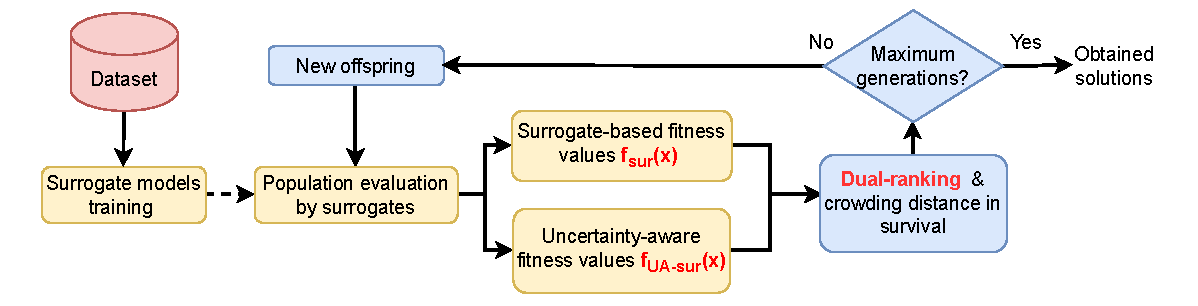
\includegraphics[width=\linewidth]{flow_chart_new.pdf}
\caption{Workflow of surrogate training and optimization. Dual-ranking is implemented by performing non-dominated sorting on solutions using both the surrogate-based function $f_{\text{sur}}$ and the uncertainty-aware function $f_{\text{UA-sur}}$.}
\label{fig: flow_chart}
\end{figure*}

\section{Method}
\subsection{Motivation}
We assume that data points $x_1, x_2, \ldots, x_n$ in a dataset $\mathcal{D}$ are drawn from an unknown distribution $p(x)$. During surrogate training, the models aim to reduce approximation errors over the dataset. However, during optimization, an off-the-shelf multi-objective optimization algorithm (e.g., NSGA-II \cite{nsga_ii}) explores the input space $\boldsymbol{X}$ to minimize the objective $\boldsymbol{f}(\boldsymbol{x})$, relying solely on the surrogate-based evaluation. When the optimizer explores unseen areas, \emph{i.e.} candidate solutions located in low-density regions of the distribution $p(x)$, the predicted objective values may be unrealistically small with high uncertainty. Such solutions may be falsely preferred by the algorithm and selected as non-dominated solutions, as illustrated in Figure~\ref{fig_1}. To address this issue, we consider both predicted values and uncertainty estimates from surrogates. The detailed workflow is shown in Figure \ref{fig: flow_chart}.

\subsection{Uncertainty-Aware Function}
For the $k$-th objective of a candidate solution $\boldsymbol{x}$, the surrogate model $\mathcal{M}_k$ outputs both a predicted value and an uncertainty estimate, whose specific forms depend on the regression model:
$\mathcal{M}_{\text{GPR},k}(\boldsymbol{x})
= \big( \mu_k(\boldsymbol{x}), \sigma_k^2(\boldsymbol{x}) \big)$,
$\mathcal{M}_{\text{QR},k}(\boldsymbol{x})
= \big( q_{\text{med},k}(\boldsymbol{x}), q_{\text{up},k}(\boldsymbol{x}) \big)$,
$\mathcal{M}_{\text{BNN},k}(\boldsymbol{x})
= \big(
q_{\text{med},k}(\boldsymbol{x}),
q_{\text{up},k}(\boldsymbol{x})
\big)$,
where the predictive mean $\mu_k(\boldsymbol{x})$ and the median prediction $q_{\text{med},k}(\boldsymbol{x})$ ($\tau=0.5$) denote the predicted value, predictive variance $\sigma_k^2(\boldsymbol{x})$ and the interval induced by the quantile estimates $q_{\text{up},k}(\boldsymbol{x})$ indicate the predictive uncertainty. For BNN, the predictive quantiles are computed from Monte Carlo samples drawn from the variational posterior over network weights.

During the fitness assignment procedure of the optimization, the fitness value of a candidate solution $\boldsymbol{x}$ is derived from the surrogate-based function $f_{\text{sur},k}$, where the results are the predictions from the surrogate model:
\begin{align}
f_{\text{sur},k}(\boldsymbol{x}) =
\begin{cases}
\mu_k(\boldsymbol{x}) & \text{(GPR)} \\
q_{\text{med},k}(\boldsymbol{x}) & \text{(QR)} \\
q_{\text{med},k}(\boldsymbol{x}) & \text{(BNN)}.
\end{cases}
\end{align}

To reduce the risk of misleading dominance judgments, we draw inspiration from the Gaussian Process Upper Confidence Bound (GP-UCB) principle~\cite{opt_ucb} and define an uncertainty-aware function $f_{\text{UA-sur},k}$. The corresponding uncertainty-aware fitness values are defined as follows:
\begin{align}
f_{\text{UA-sur},k}(\boldsymbol{x}) =
\begin{cases}
\mu_k(\boldsymbol{x}) + \alpha\, \sigma_k(\boldsymbol{x}) & \text{(GPR)} \\
q_{\text{up},k}(\boldsymbol{x}) & \text{(QR)} \\
q_{\text{up},k}(\boldsymbol{x}) & \text{(BNN)},
\end{cases}
\end{align}
where $\alpha$ is a hyperparameter that controls the degree to which solutions are penalized, while the upper quantile $q_{\text{up},k}$ characterizes the predictive uncertainty and is determined by the selected quantile level $\tau$ (\emph{e.g.} $\tau=0.9$). Larger uncertainty estimates are typically associated with less reliable fitness evaluations, which increases the risk of incorrectly judging dominance among solutions. Therefore, in minimization problems, the uncertainty-aware function penalizes large uncertainty estimates.

Inspired by the Confidence Interval Coverage Probability (CICP) indicator \cite{cicp}, we design an auto-$\alpha$ selection algorithm to select the hyperparameter $\alpha$, as shown in Algorithm~\ref{alg:find_alpha}. This hyperparameter is introduced to align the degree of penalization between uncertainty estimates provided by GPR-based models and the uncertainty-related predictions obtained from quantile-based models. The algorithm iteratively adjusts $\alpha$ on a pre-collected validation set until the empirical coverage $C(\alpha)$ of the upper confidence bound reaches the given target coverage $\tau$. Here, the target coverage $\tau$ is set equal to the selected quantile level $\tau$ used in $q_{\text{up},k}$.

\begin{algorithm}[htbp]
\caption{Auto-$\alpha$ Selection}
\label{alg:find_alpha}
\begin{algorithmic}[1]
\STATE \textbf{Input}: Validation set $(\mathbf{X}, \mathbf{y})$ with $N_{\text{val}}$ samples, surrogate model $\mathcal{M}$, target coverage $\tau$
\STATE \textbf{Output}: $\alpha$

\STATE $(\boldsymbol{\mu}, \boldsymbol{\sigma}) \leftarrow \mathcal{M}(\mathbf{X})$
\FOR{$\alpha = 0$ \TO $\alpha_{\max}$}
    \STATE $f_{\text{UA-sur}} \leftarrow \boldsymbol{\mu} + \alpha \boldsymbol{\sigma}$
    \STATE $C(\alpha) = \frac{1}{N_{\text{val}}} \sum_{i=1}^{N_{\text{val}}} \mathbb{I}\!\left(y_i \le f_{\text{UA-sur},i}\right)$
    \IF{$C(\alpha) \ge \tau$}
        \RETURN $\alpha$
    \ENDIF
\ENDFOR
\end{algorithmic}
\end{algorithm}

\begin{proposition}[Monotonicity and existence of $\alpha$]
\label{prop:alpha}
On the validation set, the empirical coverage $C(\alpha)$ is a non-decreasing function of $\alpha$, \emph{i.e.},
$
C(\alpha)
= \frac{1}{N_{\mathrm{val}}}
\sum_{i=1}^{N_{\mathrm{val}}}
\mathbb{I}\!\left(
y_i \le \mu_i + \alpha \sigma_i
\right)
$. Moreover, if there exists $\alpha^\star$ such that
$C(\alpha^\star) \ge \tau$,
Algorithm~\ref{alg:find_alpha} is guaranteed to return a feasible
$\alpha \le \alpha^\star$.
\end{proposition}


\subsection{Dual-Ranking Strategy}
In the survival step, for the $k$-th objective, each candidate solution is evaluated using both the surrogate-based function $f_{\text{sur},k}$ and the uncertainty-aware function $f_{\text{UA-sur},k}$. The dual-ranking strategy aims to select solutions with both good objective values and low uncertainty. As shown in Algorithm \ref{alg:dual_ranking}, for each candidate solution $\boldsymbol{x}$ in population $P$, the surrogate-based fitness values $f_{\text{sur}}(\boldsymbol{x}) \in \mathbb{R}^{M}$ and the uncertainty-aware fitness values $f_{\text{UA-sur}}(\boldsymbol{x}) \in \mathbb{R}^{M}$ are concatenated to form the hybrid fitness values $f_{\text{hyb}}(\boldsymbol{x}) \in \mathbb{R}^{2M}$. Non-dominated sorting is then applied to the population $P$ with updated fitness values $f_{\text{hyb}}(\boldsymbol{x}) \in \mathbb{R}^{2M}$ of each candidate solution to obtain the non-dominated fronts. 

\begin{algorithm}[htbp]
\caption{Dual-Ranking}
\label{alg:dual_ranking}
\begin{algorithmic}[1]
\STATE \textbf{Input}: Population $P$, fitness value $f_{\text{sur}}(\boldsymbol{x}) \in \mathbb{R}^{M}$ and uncertainty-aware fitness value $f_{\text{UA-sur}}(\boldsymbol{x}) \in \mathbb{R}^{M}$ of a candidate solution $\boldsymbol{x}$
\STATE \textbf{Output}: Non-dominated front $\mathcal{F}$
\FOR{each $\boldsymbol{x}$ in $P$}
  \STATE $f_{\text{hyb}}(\boldsymbol{x}) \in \mathbb{R}^{2M} 
\gets \textit{Concatenate}(f_{\text{sur}}(\boldsymbol{x}), f_{\text{UA-sur}}(\boldsymbol{x}))$
\ENDFOR
\STATE $\mathcal{F} \gets \textit{NonDominatedSorting}(P)$
\end{algorithmic}
\end{algorithm}

\begin{proposition}[Uncertainty-aware dominance judgment] \label{proposition_2}
Consider two candidate solutions $x_a$ and $x_b$ in a minimization problem.
Assume that $x_a \prec x_b$ in the surrogate-based objective space
$f_{\text{sur}}$, \emph{i.e.},
$\forall k, f_{\text{sur},k}(x_a) \le f_{\text{sur},k}(x_b)$, 
$\exists k_j, f_{\text{sur},k_j}(x_a) < f_{\text{sur},k_j}(x_b)$.
If there exists at least one objective $k$ such that
$f_{\text{UA-sur},k}(x_a) > f_{\text{UA-sur},k}(x_b)$, then $x_a \not\prec x_b$ in the hybrid objective space $f_{\text{hyb}} \in \mathbb{R}^{2M}$.
\end{proposition}

\subsection{Time Complexity}
We analyze the time complexity of the proposed dual-ranking strategy when used with NSGA-II. The standard non-dominated sorting procedure has a time complexity of $O(MN^2)$, where $N$ denotes the number of candidate solutions and $M$ the number of objectives. In the proposed dual-ranking strategy, the time complexity of concatenation operator is $O(MN)$. Non-dominated sorting is performed in the $2M$-dimensional objective space, resulting in a worst-case time complexity of $O(2MN^2)$. Therefore, total time complexity is $O(MN) + O(2MN^2) \approx O(MN^2)$. The empirical results of runtime are provided in the Section \ref{sec:runtime}.

\subsection{Benefits of Dual-Ranking}
We summarize the benefits of the proposed dual-ranking strategy. Our method jointly considers both predictive values and uncertainty-aware predictive values from surrogates to mitigate misleading rankings, while prioritizing candidate solutions that are both high-quality and reliable. Solutions with good predicted values but high uncertainty estimates or uncertainty-related predictions are penalized during ranking, preventing them from being assigned overly good ranks based solely on optimistic fitness values. Moreover, the proposed strategy can be easily integrated into non-dominated sorting, has the potential to work with other fitness assignment strategies. It can also be flexibly integrated with different surrogate models, making it suitable for offline datasets with different characteristics.

\section{Experiments}
\subsection{Experimental Setup}
\subsubsection{Benchmark Problems}
The evaluation includes 11 benchmark problems, consisting of 8 unconstrained and 3 constrained problems. The unconstrained benchmarks consist of DTLZ1–DTLZ7~\cite{opt_dtlz} with 2 objectives and 10 decision variables, and Omnitest~\cite{omnitest} with 2 objectives and 2 decision variables. The constrained benchmarks include BNH~\cite{bnh}, Truss2D~\cite{truss2d}, and Welded Beam~\cite{welded_beam}.

\subsubsection{Baseline Methods} \label{sec:baseline}
The baseline methods include Prob-RVEA, Prob-MOEA/D \cite{ddeo_rvea}, IBEA-MS \cite{ddeo_ibea}, TGPR-MO \cite{ddeo-TGPR}, and DDMOEA/GAN \cite{ddea_gan}. Other generative-based SOTA methods, including ParetoFlow~\cite{paretoflow} and Pareto-Conditioned Diffusion (PCD)~\cite{pcd}, are not compared because they typically require sufficient data to learn reliable distributions, while this work mainly focuses on surrogate models and evolutionary algorithms. Hyperparameters follow the recommended settings from the open-source code. All experiments use 30 independent runs with seeds 1–30 unless otherwise specified.

Different baseline methods adopt different optimization algorithms combined with the GPR surrogate model. As some types of optimization algorithms may be better suited for handling specific benchmark problems, the comparison experiments presented in Section~\ref{sec:results_baseline} mainly focus on overall optimization performance across all benchmarks.

\subsubsection{Offline Dataset} 
Offline data are generated by Latin Hypercube Sampling (LHS)~\cite{sampling} with a fixed random seed of 42. Following~\cite{ddeo_ibea}, the number of samples for the limited dataset is set to $11D - 1$, where $D$ denotes the number of decision variables. A relatively large dataset with 1,000 samples is also evaluated, with detailed results reported in the Supplementary Material.

\subsubsection{Surrogate Models}
For GPR, the Gaussian kernel \cite{gaussian_kernel} and ARD Mat\'ern 5/2 kernel \cite{kernel_Matern_52} are used. In some test cases, to avoid constant predictions, the variance of the Gaussian noise is set to a very small value of $10^{-6}$. QR is implemented using AutoGluon-Tabular \cite{ml_autogluon}, with quantile levels of 0.5 and 0.9, and a fixed random seed of 42. BNN is implemented by Pyro~\cite{pyro} and employs the AutoDiagonalNormal for variational inference. The BNN model uses a hidden dimension of 16, an initial learning rate of $10^{-3}$, the Adam optimizer~\cite{adam}. The number of training epochs is tuned with early stopping mechanism for each benchmark problem. Other settings are reported in the Supplementary Material.

\subsubsection{Optimization Algorithms}
The optimization framework is implemented using pymoo \cite{pymoo}. The population size is set to 100, and the maximum number of generations is 100, resulting in a total of 10,000 fitness evaluations. For the reproduction operators, Simulated Binary Crossover (SBX) \cite{opt-sbx} is applied with a crossover probability of 1.0 and a distribution factor of $\eta = 20$. Polynomial mutation \cite{nsga_ii} is employed with a mutation probability of $1/D$ and the same distribution factor. 

\subsubsection{Performance Indicators}
Surrogate prediction performance is evaluated using Mean Squared Error (MSE) and CICP~\cite{cicp}, with detailed results provided in the Supplementary Material. MSE measures the difference between predictions $\hat{y}$ and ground truth $y$, while CICP evaluates uncertainty estimates by computing the fraction of function values that fall inside the corresponding confidence intervals. 

For optimization, the indicators include MSE, Inverted Generational Distance Plus (IGD+) \cite{igd_plus} and Hypervolume (HV) \cite{hypervolume}. The MSE indicator measures the difference between the real evaluations and the surrogate-based evaluations. Both IGD+ and HV indicators are employed to evaluate the optimization results of real evaluations, since the surrogate-based evaluations may introduce errors. The IGD+ indicator is available as the PF is known on synthetic problems. For the HV indicator, Min-Max normalization \cite{indicator} is applied, and the bounds are selected based on the benchmark \cite{benchmark} and valid ranges, with details provided in the Supplementary Material. The reference point is $(1.1, 1.1)$. We adopt the Wilcoxon signed-rank test \cite{wilcoxon} for statistical testing.

\subsection{Surrogate Model Prediction Performance}
The results of surrogate model prediction performance are summarized in this section, while detailed results and discussions for both the limited dataset and the 1,000-sample dataset are provided in the Supplementary Material. The GPR (Mat\'ern) model generally achieves lower prediction errors than the GPR (RBF) model across most benchmark problems. The GPR (RBF) model occasionally yields slightly higher CICP values but increased MSE. QR consistently delivers high CICP values across nearly all cases, demonstrating robust uncertainty estimates despite relatively larger MSE. The BNN model shows variability in both prediction accuracy and uncertainty estimates. 

These observations indicate a trade-off between prediction accuracy and reliable uncertainty estimates, which motivates the uncertainty-aware function with dual-ranking strategy adopted in this work.

\subsection{Ablation Study and Sensitivity Analysis}
Ablation and sensitivity analyses are conducted on 11 benchmark problems by comparing each baseline with its dual-ranking variant. For sensitivity analysis, $\tau$ is set to $0.80$, $0.90$, and $0.95$ as the target coverage rate for GPR-based models and the quantile level for AutoGluon-QR and BNN models. Due to page limits, Table~\ref{tab:opt_counts} reports the summary comparison counts, with detailed results provided in the Supplementary Material.

\begin{table*}[htbp]
\caption{Ablation study and sensitivity analysis results across 11 benchmark problems, for different surrogate models combined with the NSGA-II (omitted). Each method is evaluated under different Dual-Ranking (DR) settings for sensitivity analysis. 
All indicators are optimization performance indicators. For each indicator, ``$+$/$=$/$-$'' denotes better/comparable/worse performance than the corresponding baseline without the dual-ranking strategy, based on the statistical test results.}
\label{tab:opt_counts}
\centering
\begin{tabular}{l|ccc|ccc|ccc}
\hline
\multirow{2}{*}{Methods} 
& \multicolumn{3}{c|}{MSE} 
& \multicolumn{3}{c|}{IGD+} 
& \multicolumn{3}{c}{HV} \\
 & $+$ & $=$ & $-$ & $+$ & $=$ & $-$ & $+$ & $=$ & $-$ \\
\hline
GPR (RBF) + DR ($\tau{=}0.80$) & 3 & 6 & 2 & 1 & 9 & 1 & 2 & 7 & 2 \\
GPR (RBF) + DR ($\tau{=}0.90$) & 5 & 4 & 2 & 4 & 6 & 1 & 5 & 5 & 1 \\
GPR (RBF) + DR ($\tau{=}0.95$) & 4 & 5 & 2 & 2 & 6 & 3 & 3 & 6 & 2 \\

\hline
GPR (Mat\'ern) + DR ($\tau{=}0.80$) & 3 & 5 & 3 & 2 & 8 & 1 & 4 & 5 & 2 \\
GPR (Mat\'ern) + DR ($\tau{=}0.90$) & 3 & 5 & 3 & 4 & 6 & 1 & 5 & 5 & 1 \\
GPR (Mat\'ern) + DR ($\tau{=}0.95$) & 3 & 5 & 3 & 4 & 5 & 2 & 5 & 5 & 1 \\
\hline
QR + DR ($\tau{=}0.80$) & 4 & 3 & 4 & 8 & 3 & 0 & 8 & 3 & 0 \\
QR + DR ($\tau{=}0.90$) & 4 & 3 & 4 & 7 & 4 & 0 & 8 & 3 & 0 \\
QR + DR ($\tau{=}0.95$) & 3 & 4 & 4 & 7 & 4 & 0 & 8 & 2 & 1 \\
\hline
BNN + DR ($\tau{=}0.80$) & 1 & 9 & 1 & 2 & 8 & 1 & 3 & 7 & 1 \\
BNN + DR ($\tau{=}0.90$) & 5 & 5 & 1 & 5 & 4 & 2 & 4 & 5 & 2 \\
BNN + DR ($\tau{=}0.95$) & 3 & 7 & 1 & 4 & 5 & 2 & 4 & 5 & 2 \\
\hline
\end{tabular}
\end{table*}

Overall, the results indicate that the dual-ranking strategy is robust to the choice of $\tau$ within a reasonable range. The value of $\tau$ mainly affects optimization performance across different problems, rather than the reliability of surrogate-based evaluations. The improvements are more evident for IGD+ and HV than for MSE, especially for QR, where the dual-ranking variants achieve gains across different $\tau$ settings. These results also suggest that a moderate value, \emph{i.e.}, $\tau=0.90$, provides a good trade-off and is therefore used as the default setting in the following experiments.

We also conduct an ablation study comparing the dual-ranking strategy with the sole use of $f_{\text{UA-sur}}$, with the results reported in the Supplementary Material. These results show that the dual-ranking variants achieve comparable performance for the GPR-based methods and perform better in more cases for QR and BNN.

\subsection{Runtime Evaluation and Generalization to MOEAs} \label{sec:runtime}
These experiments evaluate the runtime of different methods with and without dual-ranking, as well as the generalization ability of dual-ranking across different MOEAs. Summary results are reported here, and detailed empirical results are provided in the Supplementary Material.

The mean runtime difference indicates that the proposed dual-ranking strategy introduces only minor additional computational cost, below 1.5\%.

The dual-ranking strategy is further integrated with Nondominated Sorting Genetic Algorithm III (NSGA-III)~\cite{nsga3} and the S-Metric Selection Evolutionary Multiobjective Algorithm (SMS-EMOA)~\cite{sms_emoa}. The results show that dual-ranking combined with NSGA-III achieves performance comparable to that with NSGA-II, while its improvement with SMS-EMOA is relatively smaller.

\subsection{Performance Comparison with Baseline Methods} \label{sec:results_baseline}
This experiment compares the optimization performance of the proposed dual-ranking–based methods with baseline offline data-driven MOO methods on 8 unconstrained benchmark problems, as most baseline methods cannot handle constraints. Table~\ref{tab:opt_baseline_ranks} summarizes the overall ranking results. The ranks are computed for each performance indicator on each benchmark problem. The mean and standard deviation of the overall ranks are then calculated based on these detailed ranks.

\begin{table*}[htbp]
\caption{Ranking results (mean $\pm$ std.). Our method uses NSGA-II with dual-ranking (DR), where $\tau=0.9$. \textbf{Bold} and \underline{underline} denote the best and second-best results, respectively.}
\label{tab:opt_baseline_ranks}
\centering
\begin{tabular}{lcc}
\toprule
Methods 
& Limited dataset $\downarrow$
& 1,000 samples $\downarrow$ \\
\midrule
Prob-RVEA          
& 5.17 $\pm$ 2.56 
& 7.71 $\pm$ 1.27 \\
Prob-MOEA/D        
& 6.12 $\pm$ 3.02 
& 7.21 $\pm$ 1.22 \\
IBEA-MS            
& \underline{3.38 $\pm$ 2.66} 
& 3.48 $\pm$ 1.89 \\
TGPR-MO            
& 3.50 $\pm$ 1.78 
& 4.25 $\pm$ 1.94 \\
DDMOEA/GAN         
& 6.00 $\pm$ 3.21 
& 5.92 $\pm$ 3.17 \\
GPR(RBF)+DR        
& 4.67 $\pm$ 1.57 
& \underline{2.50 $\pm$ 1.72} \\
\textbf{GPR(Mat\'ern)+DR} 
& \textbf{3.25 $\pm$ 1.51} 
& \textbf{2.42 $\pm$ 1.84} \\
QR+DR              
& 5.17 $\pm$ 1.80 
& 3.50 $\pm$ 1.56 \\
BNN+DR             
& 6.38 $\pm$ 2.14 
& 6.04 $\pm$ 2.20 \\
\bottomrule
\end{tabular}
\end{table*}

As stated in Section \ref{sec:baseline} Baseline Methods, we focus on the overall optimization performance. Among all compared methods, GPR(Mat\'ern)+DR achieves the competitive overall rank. These results indicate that incorporating the dual-ranking strategy into GPR with a Mat\'ern kernel yields competitive optimization performance.

The standard deviation of overall ranks further highlights the robustness advantage of the proposed dual-ranking strategy. Although dual-ranking–based methods do not achieve the best performance on each benchmark problem, all surrogates incorporating the dual-ranking strategy exhibit relatively small standard deviations. In contrast, while IBEA-MS or DDMOEA/GAN may perform competitively on certain problems, their larger standard deviations indicate weaker robustness across different benchmarks. Dual-ranking–based methods benefit from increased training data, as evidenced by their improved mean ranks in the 1,000-sample setting. In contrast, some baseline methods (e.g., IBEA-MS) perform relatively well under limited data but are surpassed by dual-ranking–based GPR methods as the dataset size increases. 

\section{Real-World Case Study}
We adopt the flexible building space usage optimization problem~\cite{building_opt2}, which is formulated as a MOP that jointly optimizes energy consumption and thermal comfort. Since building energy consumption cannot be directly calculated, surrogate models are required for prediction. The training dataset contains 288 samples (1 day) from a building dataset~\cite{dataset-1} to simulate real-world limited offline dataset settings. Other initial settings and optimization results are provided in the Supplementary Material.

Since real evaluations are unavailable for this real-world problem, we use HV as the performance indicator, and its values are computed from surrogate-based evaluations, as shown in Table~\ref{tab:real_world}. The HV results show that incorporating dual-ranking may improve solution quality. We also observe that the dual-ranking variants provide more potential solutions than the standard methods.

\begin{table*}[htbp]
\centering
\caption{Comparison of HV values in the real-world case study. \textbf{Bold} indicates the larger value.}
\label{tab:real_world}
\begin{tabular}{lcccc}
\toprule
Methods & GPR (RBF) & GPR (Mat\'ern) & QR & BNN \\
\midrule
Standard
& \textbf{0.1064} & 0.1017 & 0.1001 & 0.1452 \\
Dual-ranking variant
& 0.1060 & \textbf{0.1019} & \textbf{0.1003} & \textbf{0.1459} \\
\bottomrule
\end{tabular}
\end{table*}

\section{Conclusion}
In this work, we propose a dual-ranking strategy that jointly leverages surrogate predictions and uncertainty estimates to mitigate misleading rankings during optimization. The prediction experiments motivate our design of the uncertainty-aware function used in dual-ranking. The ablation study shows that the dual-ranking strategy improves the reliability of surrogate-based evaluations and shows limited sensitivity to the target coverage rate or quantile level $\tau$. A moderate value, such as $\tau=0.90$, provides a balanced trade-off. The dual-ranking strategy introduces only minor computational cost and can be generalized to other optimization algorithms. Baseline comparison experiments show that GPR with a Mat\'ern kernel and the proposed dual-ranking strategy achieves the competitive overall performance. Moreover, the relatively small standard deviations across dual-ranking-based methods indicate improved robustness. The real-world case study illustrates the practical potential of integrating the uncertainty-aware data-driven methods into building optimization.

In future work, we plan to verify the methods on many-objective optimization scenarios ($M > 3$). We will also investigate more real-world cases, and online settings with continuously arriving data, where measurement errors exist in real-time data streams.


\bibliographystyle{plainnat}
\bibliography{reference}


%%%%%%%%%%%%%%%%%%%%%%%%%%%%%%%%%%%%%%%%%%%%%%%%%%%%%%%%%%%%

\appendix

\section{Technical appendices and supplementary material}

\subsection{Proofs}

\begin{proof}[Proof of Proposition~\ref{prop:alpha}]
For any $\alpha_1 \le \alpha_2$ and any validation sample $i$, $\sigma_i \ge 0$, we have
\[
\mu_i + \alpha_1 \sigma_i \le \mu_i + \alpha_2 \sigma_i .
\]
Therefore, if 
\[
y_i \le \mu_i + \alpha_1 \sigma_i,
\]
then also
\[
y_i \le \mu_i + \alpha_2 \sigma_i.
\]
Thus, the $C(\alpha)$ is non-decreasing.

If Algorithm~\ref{alg:find_alpha} searches candidate values of $\alpha$ in 
ascending order and returns the first value satisfying $C(\alpha)\ge \tau$, 
then, whenever the search set contains a feasible value $\alpha^\star$, the 
algorithm must return a feasible value $\alpha \le \alpha^\star$.
\end{proof}

\begin{proof}[Proof of Proposition~\ref{proposition_2}]
By definition, the hybrid objective vector is
\[
f_{\mathrm{hyb}}(x)
=
\left(
f_{\mathrm{sur},1}(x),\ldots,f_{\mathrm{sur},M}(x),
f_{\mathrm{UA\text{-}sur},1}(x),\ldots,f_{\mathrm{UA\text{-}sur},M}(x)
\right).
\]
For a minimization problem, $x_a \prec x_b$ in the hybrid objective space only if 
\[
\forall k, f_{\text{hyb},k}(x_a) \le f_{\text{hyb},k}(x_b), 
\exists k_j, f_{\text{hyb},k_j}(x_a) < f_{\text{hyb},k_j}(x_b).
\]
However, if there exists an objective $k$ such that
\[
f_{\mathrm{UA\text{-}sur},k}(x_a)
>
f_{\mathrm{UA\text{-}sur},k}(x_b),
\]
then the dominance condition in the hybrid objective space is violated,
and thus $x_a \not\prec x_b$.
\end{proof}

\subsection{Experimental Settings}
The experiments were conducted on Google Colab using an Intel Xeon CPU @ 2.20GHz, and .

The Hypervolume (HV) \cite{hypervolume} reference point $(1.1, 1.1)$ and the bounds \cite{benchmark} for Min-Max normalization \cite{indicator} are shown in Table~\ref{tab: reference_points}. 

\begin{table*}[htbp]
\caption{Bounds for Min-Max normalization and hypervolume reference points.}
\label{tab: reference_points}
\centering
\begin{tabular}{lcccc}
\toprule
&Problem &Min &Max &Reference point \\
\midrule
&DTLZ1~\cite{opt_dtlz} &(0,0) &(552.30,568.36) &(1.10, 1.10) \\
&DTLZ2 &(0,0) &(2.78,2.93) &(1.10, 1.10) \\
&DTLZ3 &(0,0) &(1605.54,1670.48) &(1.10, 1.10) \\
&DTLZ4 &(0,0) &(2.83,2.78) &(1.10, 1.10) \\
&DTLZ5 &(0,0) &(2.61,2.70) &(1.10, 1.10) \\
&DTLZ6 &(0,0) &(9.78,9.78) &(1.10, 1.10) \\
&DTLZ7 &(0,0) &(1.10,33.43) &(1.10, 1.10) \\
&BNH~\cite{bnh} &(0,5) &(140,50) &(1.10, 1.10) \\
&Truss2D~\cite{truss2d} &(0,0) &(0.10,1e5) &(1.10, 1.10) \\
&Welded Beam~\cite{welded_beam} &(0,0) &(35,0.10) &(1.10, 1.10) \\
\bottomrule
\end{tabular}


\end{table*}

\subsection{Surrogate Model Prediction Performance}
The prediction performance comparison of different surrogate models across 11 benchmark problems with limited training data ($11D-1$ samples) is presented in Table~\ref{tab:prediction}, while the results obtained with 1,000 training samples are shown in Table~\ref{tab:prediction_1000}. We use Mean Squared Error (MSE) to evaluate prediction accuracy and Confidence Interval Coverage Probability (CICP)~\cite{cicp} to assess uncertainty estimation performance.

\subsubsection{Prediction Results with Limited Training Data}
From Table~\ref{tab:prediction}, the Gaussian Process Regression (GPR) with Mat\'ern kernel surrogate \cite{kernel_Matern_52} achieves lower MSE than GPR (RBF) surrogate \cite{gaussian_kernel} on many problems, including DTLZ2–DTLZ7 and engineering problems. In contrast, GPR (RBF) tends to achieve slightly higher or comparable CICP values on some problems, but often increases the prediction errors. QR \cite{ml_autogluon} consistently delivers high CICP values across nearly all cases, demonstrating robust uncertainty estimations despite relatively larger MSE. The BNN \cite{bnn} surrogate exhibits competitive CICP values on some problems but degraded prediction accuracy or CICP values on others. These results show a trade-off between prediction accuracy and reliable uncertainty estimation across all problems.

\begin{table*}[!h]
\caption{Prediction performance comparison of different surrogates across 11 benchmark problems.}
\label{tab:prediction}
\centering
\resizebox{\linewidth}{!}{
\begin{tabular}{lcccccccccccc}
\hline
Surrogates
& \multicolumn{2}{c}{DTLZ1}
& \multicolumn{2}{c}{DTLZ2}
& \multicolumn{2}{c}{DTLZ3}
& \multicolumn{2}{c}{DTLZ4}
& \multicolumn{2}{c}{DTLZ5}
& \multicolumn{2}{c}{DTLZ6} \\
\cline{2-13}
& MSE & CICP
& MSE & CICP
& MSE & CICP
& MSE & CICP
& MSE & CICP
& MSE & CICP \\
\hline
GPR (RBF)
& $4.67\mathrm{E}{+03}$ & 88.50\%
& $2.78\mathrm{E}{-02}$ & 76.50\%
& $2.69\mathrm{E}{+04}$ & 87.50\%
& $3.89\mathrm{E}{-02}$ & 84.00\%
& $2.78\mathrm{E}{-02}$ & 76.50\%
& $1.06\mathrm{E}{-02}$ & 53.50\% \\
GPR (Mat\'ern)
& $4.81\mathrm{E}{+03}$ & 88.00\%
& $1.87\mathrm{E}{-02}$ & 73.50\%
& $2.68\mathrm{E}{+04}$ & 87.50\%
& $1.94\mathrm{E}{-02}$ & 90.00\%
& $1.87\mathrm{E}{-04}$ & 73.50\%
& $6.92\mathrm{E}{-03}$ & 74.00\% \\
QR
& $5.01\mathrm{E}{+03}$ & 92.50\%
& $2.45\mathrm{E}{-02}$ & 94.00\%
& $2.89\mathrm{E}{+04}$ & 89.00\%
& $3.21\mathrm{E}{-02}$ & 92.00\%
& $2.45\mathrm{E}{-02}$ & 94.00\%
& $5.97\mathrm{E}{-02}$ & 94.00\% \\
BNN
& $5.00\mathrm{E}{+03}$ & 72.00\%
& $3.01\mathrm{E}{-02}$ & 80.00\%
& $2.83\mathrm{E}{+04}$ & 66.50\%
& $4.43\mathrm{E}{-02}$ & 76.00\%
& $2.99\mathrm{E}{-02}$ & 79.00\%
& $1.39\mathrm{E}{-02}$ & 83.00\% \\
\hline
\multicolumn{13}{c}{} \\
\hline
Surrogates
& \multicolumn{2}{c}{DTLZ7}
& \multicolumn{2}{c}{Omnitest}
& \multicolumn{2}{c}{BNH}
& \multicolumn{2}{c}{Truss2D}
& \multicolumn{2}{c}{Welded Beam}
& \multicolumn{2}{c}{} \\
\cline{2-11}
& MSE & CICP
& MSE & CICP
& MSE & CICP
& MSE & CICP
& MSE & CICP
&  &  \\
\hline
GPR (RBF)
& $4.92\mathrm{E}{-02}$ & 95.50\%
& $8.33\mathrm{E}{-01}$ & 85.00\%
& $1.23\mathrm{E}{-07}$ & 100.00\%
& $3.15\mathrm{E}{+12}$ & 91.00\%
& $4.20\mathrm{E}{+02}$ & 91.00\% \\
GPR (Mat\'ern)
& $3.34\mathrm{E}{-08}$ & 100.00\%
& $8.52\mathrm{E}{-01}$ & 76.00\%
& $2.02\mathrm{E}{-05}$ & 100.00\%
& $3.11\mathrm{E}{+12}$ & 94.00\%
& $4.26\mathrm{E}{+02}$ & 93.00\% \\
QR
& $1.21\mathrm{E}{-01}$ & 91.00\%
& $1.24\mathrm{E}{+00}$ & 78.50\%
& $1.98\mathrm{E}{+01}$ & 79.50\%
& $2.73\mathrm{E}{+12}$ & 97.50\%
& $6.39\mathrm{E}{+02}$ & 91.00\% \\
BNN
& $1.13\mathrm{E}{-01}$ & 65.50\%
& $1.27\mathrm{E}{+00}$ & 53.50\%
& $1.22\mathrm{E}{+01}$ & 95.00\%
& $2.62\mathrm{E}{+12}$ & 96.50\%
& $6.01\mathrm{E}{+02}$ & 92.50\% \\
\hline
\end{tabular}
}

\end{table*}

\subsubsection{Prediction Results with 1000 Training Data}
From Table~\ref{tab:prediction_1000}, all surrogate models benefit from the larger dataset compared to the limited data setting, with substantially reduced MSE and improved CICP values across almost all benchmark problems. The GPR (Mat\'ern) surrogate generally achieves lower MSE and higher or comparable CICP values than the GPR (RBF) surrogate, particularly on DTLZ2, DTLZ4–DTLZ7, Truss2D and Welded Beam. QR surrogate maintains relatively high and stable CICP values on most benchmark problems but exhibits larger prediction errors compared to GPR-based models. The BNN surrogate shows improved CICP values on several problems with 1000 training data, however, its prediction accuracy  and CICP values remain more variable than those of other surrogates.

Overall, increasing the training dataset size to 1000 samples improves both prediction accuracy and CICP values for all surrogates. Despite the performance improvement, the relative performance trends among different surrogates remain consistent with those observed under limited training data.

\begin{table*}[htbp]
\caption{Prediction performance comparison of different surrogates trained on 1000 samples across 11 benchmark problems.}
\label{tab:prediction_1000}
\centering
\resizebox{\linewidth}{!}{
\begin{tabular}{lcccccccccccc}
\hline
Surrogates
& \multicolumn{2}{c}{DTLZ1}
& \multicolumn{2}{c}{DTLZ2}
& \multicolumn{2}{c}{DTLZ3}
& \multicolumn{2}{c}{DTLZ4}
& \multicolumn{2}{c}{DTLZ5}
& \multicolumn{2}{c}{DTLZ6} \\
\cline{2-13}
& MSE & CICP
& MSE & CICP
& MSE & CICP
& MSE & CICP
& MSE & CICP
& MSE & CICP \\
\hline
GPR (RBF) (1000)
& $4.46\mathrm{E}{+03}$ & 88.50\%
& $6.05\mathrm{E}{-09}$ & 98.00\%
& $2.59\mathrm{E}{+04}$ & 88.00\%
& $4.95\mathrm{E}{-04}$ & 88.00\%
& $6.05\mathrm{E}{-09}$ & 98.00\%
& $3.53\mathrm{E}{-03}$ & 82.00\% \\
GPR (Mat\'ern) (1000)
& $4.43\mathrm{E}{+03}$ & 89.00\%
& $5.87\mathrm{E}{-06}$ & 99.50\%
& $2.57\mathrm{E}{+04}$ & 88.00\%
& $5.67\mathrm{E}{-04}$ & 96.00\%
& $5.87\mathrm{E}{-06}$ & 99.50\%
& $2.58\mathrm{E}{-03}$ & 89.00\% \\
QR
& $4.51\mathrm{E}{+03}$ & 86.50\%
& $3.56\mathrm{E}{-03}$ & 90.00\%
& $2.54\mathrm{E}{+04}$ & 85.50\%
& $4.06\mathrm{E}{-03}$ & 91.50\%
& $3.56\mathrm{E}{-03}$ & 90.00\%
& $9.34\mathrm{E}{-03}$ & 96.00\% \\
BNN
& $4.65\mathrm{E}{+03}$ & 75.00\%
& $2.59\mathrm{E}{-02}$ & 83.50\%
& $2.57\mathrm{E}{+04}$ & 64.00\%
& $3.59\mathrm{E}{-02}$ & 77.00\%
& $2.49\mathrm{E}{-02}$ & 74.00\%
& $7.30\mathrm{E}{-03}$ & 96.50\% \\
\hline
\multicolumn{13}{c}{} \\
\hline
Surrogates
& \multicolumn{2}{c}{DTLZ7}
& \multicolumn{2}{c}{Omnitest}
& \multicolumn{2}{c}{BNH}
& \multicolumn{2}{c}{Truss2D}
& \multicolumn{2}{c}{Welded Beam}
& \multicolumn{2}{c}{} \\
\cline{2-11}
& MSE & CICP
& MSE & CICP
& MSE & CICP
& MSE & CICP
& MSE & CICP
&  &  \\
\hline
GPR (RBF) (1000)
& $2.76\mathrm{E}{-10}$ & 100.00\%
& $2.19\mathrm{E}{-10}$ & 100.00\%
& $1.78\mathrm{E}{-07}$ & 100.00\%
& $2.74\mathrm{E}{+12}$ & 99.50\%
& $9.41\mathrm{E}{+01}$ & 98.00\% \\
GPR (Mat\'ern) (1000)
& $2.48\mathrm{E}{-10}$ & 99.50\%
& $2.26\mathrm{E}{-06}$ & 100.00\%
& $4.74\mathrm{E}{-07}$ & 100.00\%
& $2.46\mathrm{E}{+12}$ & 98.00\%
& $9.44\mathrm{E}{+00}$ & 98.50\% \\
QR
& $4.97\mathrm{E}{-02}$ & 90.00\%
& $5.12\mathrm{E}{-03}$ & 91.00\%
& $2.25\mathrm{E}{-01}$ & 98.50\%
& $1.19\mathrm{E}{+12}$ & 97.50\%
& $8.24\mathrm{E}{+01}$ & 52.50\% \\
BNN
& $7.49\mathrm{E}{-02}$ & 88.00\%
& $1.52\mathrm{E}{-03}$ & 70.00\%
& $5.49\mathrm{E}{+00}$ & 99.50\%
& $2.73\mathrm{E}{+12}$ & 96.50\%
& $3.40\mathrm{E}{+01}$ & 99.00\% \\
\hline
\end{tabular}
}

\end{table*}

\subsection{Ablation Study and Sensitivity Analysis}
The optimization performance indicators include MSE, Inverted Generational Distance Plus (IGD+)~\cite{igd_plus}, and HV~\cite{hypervolume}. For both MSE and IGD+, smaller values indicate better performance, whereas larger HV values are preferred. As all surrogates are combined with the same optimization algorithm Non-dominated Sorting Genetic Algorithm II (NSGA-II), this is omitted in the table.

\subsubsection{Ablation Study with Limited Training Data}
The ablation study results of optimization performance comparisons and sensitivity analysis with limited training data ($11D-1$ samples) are presented in Table~\ref{tab:opt}. The Dual-Ranking (DR) strategy consistently improves or preserves optimization performance for all surrogate models combined with NSGA-II. These improvements are not limited to a specific problem but are observed across both unconstrained and constrained benchmark problems.

For the GPR (RBF) method with dual-ranking strategy, MSE is reduced on all DTLZ problems and on 3 out of 4 remaining problems, while performance remains unchanged or only marginally affected in the other cases. IGD+ is improved in 4 out of 7 DTLZ problems and in 3 out of 4 other problems, with no severe degradation observed. The HV metric is largely preserved across DTLZ problems and significantly improved in 2 out of 4 other problems, particularly on constrained benchmarks such as BNH and Truss2D. Overall, these results indicate that dual-ranking strategy substantially enhances solution quality for the GPR (RBF) method.

For GPR with the Mat\'ern kernel, the baseline model already exhibits strong performance on several problems. Dual-ranking strategy further improves optimization outcomes. Across all benchmark problems, both MSE and IGD+ are reduced in 6 out of 11 cases, while HV performance is improved or preserved in many problems. In particular, constrained benchmarks benefit the most from the dual-ranking strategy, where MSE and IGD+ are consistently reduced while HV is improved. This demonstrates that dual-ranking strategy remains effective even when combined with a well-performing surrogate model.

For the QR method, the dual-ranking strategy produces consistent improvements across almost all benchmark problems. MSE is reduced in 7 out of 11 cases and IGD+ is reduced in 8 out of 11 cases. HV is improved or preserved in at least 10 problems. These results show that dual-ranking strategy effectively improves or preserves the optimization performance.

The BNN model shows variable performance in the baseline setting. After incorporating dual-ranking strategy, optimization results become substantially more stable. On unconstrained problems, dual-ranking strategy improves IGD+ and HV in most cases, even when MSE improvements are limited. For constrained problems, dual-ranking strategy preserves or improves solution quality. This indicates enhanced robustness across both unconstrained and constrained scenarios.

Across all methods, these improvement patterns remain consistent under different dual-ranking parameter settings. No single parameter choice leads to performance degradation across all problems. In most cases, intermediate to large parameter values (e.g., $\tau=0.90$ for GPR-based models and $\tau=0.90$ for QR and BNN) achieve a good balance. Overall, the results confirm that the proposed dual-ranking strategy delivers robust performance gains across diverse problems without requiring careful hyperparameter tuning.

\begin{table*}[htbp]
\caption{Ablation study and sensitivity analysis of optimization performance comparisons across 11 benchmark problems. Each method is evaluated under different Dual-Ranking (DR) settings (the target coverage rate $\tau = 0.80, 0.90, 0.95$ or the quantile level $\tau = 0.80, 0.90, 0.95$) for sensitivity analysis. \textbf{Bold} indicates improvement over the baseline without DR, and \underline{underline} indicates equal performance.}
\label{tab:opt}
\centering
\resizebox{\linewidth}{!}{
\begin{tabular}{l ccc ccc ccc ccc ccc ccc}
\hline
Methods
& \multicolumn{3}{c}{DTLZ1}
& \multicolumn{3}{c}{DTLZ2}
& \multicolumn{3}{c}{DTLZ3}
& \multicolumn{3}{c}{DTLZ4}
& \multicolumn{3}{c}{DTLZ5}
& \multicolumn{3}{c}{DTLZ6} \\
\cmidrule(lr){2-4} \cmidrule(lr){5-7} \cmidrule(lr){8-10} \cmidrule(lr){11-13} \cmidrule(lr){14-16} \cmidrule(lr){17-19}
& MSE & IGD+ & HV
& MSE & IGD+ & HV
& MSE & IGD+ & HV
& MSE & IGD+ & HV
& MSE & IGD+ & HV
& MSE & IGD+ & HV \\
\hline
GPR (RBF)
& 1.01E+04 & 1.08E+02 & 1.15
& 5.92E-02 & 5.49E-01 & 0.96
& 2.53E+04 & 4.25E+02 & 1.11
& 2.70E-01 & 4.50E-01 & 0.85
& 5.92E-02 & 5.43E-01 & 0.92
& 1.52E+00 & 4.40E+00 & 0.95 \\
GPR + DR ($\tau=0.80$)
& \textbf{9.74E+03} & 1.11E+02 & \underline{1.15}
& \textbf{5.27E-02} & \textbf{5.32E-01} & \underline{0.96}
& 2.58E+04 & \textbf{3.92E+02} & \textbf{1.12}
& \textbf{1.98E-01} & 4.56E-01 & 0.83
& \textbf{5.27E-02} & \textbf{5.28E-01} & \underline{0.92}
& \textbf{1.06E+00} & 4.65E+00 & 0.93 \\
GPR + DR ($\tau=0.90$)
& \textbf{9.43E+03} & 1.16E+02 & 1.14
& \textbf{5.44E-02} & \textbf{5.17E-01} & \textbf{0.97}
& \textbf{2.28E+04} & 4.18E+02 & \underline{1.11}
& \textbf{2.08E-01} & 4.73E-01 & 0.83
& \textbf{5.44E-02} & \textbf{5.12E-01} & \textbf{0.93}
& \textbf{6.32E-01} & 4.98E+00 & 0.89 \\
GPR + DR ($\tau=0.95$)
& \textbf{8.36E+03} & 1.25E+02 & 1.13
& \textbf{5.11E-02} & \textbf{5.21E-01} & \textbf{0.97}
& 2.57E+04 & \textbf{4.12E+02} & \textbf{1.12}
& \textbf{1.78E-01} & 4.59E-01 & 0.82
& \textbf{5.11E-02} & \textbf{5.19E-01} & \textbf{0.93}
& \textbf{3.68E-01} & 5.29E+00 & 0.86 \\
\hline
GPR (Mat\'ern)
& 9.59E+03 & 1.19E+02 & 1.14
& 1.54E-02 & 8.32E-02 & 1.09
& 2.54E+04 & 3.97E+02 & 1.12
& 1.85E-01 & 4.64E-01 & 0.79
& 1.54E-02 & 8.24E-02 & 1.08
& 2.37E+00 & 4.12E+00 & 0.98 \\
GPR + DR ($\tau=0.80$)
& \textbf{8.44E+03} & 1.25E+02 & 1.13
& 1.77E-02 & \textbf{7.35E-02} & \textbf{1.10}
& \textbf{2.38E+04} & 4.19E+02 & 1.11
& 2.15E-01 & 4.65E-01 & \textbf{0.80}
& 1.77E-02 & \textbf{7.35E-02} & \underline{1.08}
& \textbf{1.81E+00} & 4.36E+00 & 0.95 \\
GPR + DR ($\tau=0.90$)
& \textbf{7.94E+03} & 1.33E+02 & 1.12
& 2.00E-02 & \textbf{6.61E-02} & \textbf{1.10}
& \textbf{2.27E+04} & 4.24E+02 & 1.11
& 2.43E-01 & \textbf{4.43E-01} & \textbf{0.80}
& 2.00E-02 & \textbf{6.68E-02} & \underline{1.08}
& \textbf{1.45E+00} & 4.51E+00 & 0.94 \\
GPR + DR ($\tau=0.95$)
& \textbf{7.61E+03} & 1.24E+02 & 1.13
& 1.95E-02 & \textbf{6.15E-02} & \textbf{1.10}
& \textbf{2.24E+04} & 4.29E+02 & 1.11
& 2.35E-01 & \textbf{4.21E-01} & \textbf{0.80}
& 1.95E-02 & \textbf{6.21E-02} & \underline{1.08}
& \textbf{1.17E+00} & 4.68E+00 & 0.92 \\
\hline
QR
& 8.06E+03 & 1.85E+02 & 1.04
& 2.15E-01 & 2.00E-01 & 1.06
& 3.45E+04 & 4.51E+02 & 1.11
& 9.47E-01 & 5.73E-01 & 0.88
& 2.15E-01 & 2.08E-01 & 1.03
& 1.97E-01 & 6.70E+00 & 0.68 \\
QR + DR ($q=0.80$)
& \textbf{6.86E+03} & 1.93E+02 & 1.02
& \textbf{5.95E-02} & \textbf{1.40E-01} & \textbf{1.07}
& 3.91E+04 & \textbf{4.46E+02} & 1.10
& \textbf{5.61E-01} & \textbf{3.24E-01} & \textbf{0.93}
& \textbf{5.95E-02} & \textbf{1.44E-01} & \textbf{1.05}
& 2.28E-01 & \textbf{6.61E+00} & \textbf{0.69} \\
QR + DR ($\tau=0.90$)
& \textbf{6.63E+03} & 2.06E+02 & 1.01
& \textbf{5.23E-02} & \textbf{1.16E-01} & \textbf{1.08}
& 3.85E+04 & 4.89E+02 & 1.10
& \textbf{6.00E-01} & \textbf{1.96E-01} & \textbf{1.01}
& \textbf{5.23E-02} & \textbf{1.18E-01} & \textbf{1.06}
& 2.15E-01 & \textbf{6.66E+00} & \underline{0.68} \\
QR + DR ($\tau=0.95$)
& \textbf{6.69E+03} & 2.08E+02 & 1.01
& \textbf{4.94E-02} & \textbf{1.23E-01} & \textbf{1.08}
& 3.47E+04 & 4.62E+02 & \underline{1.11}
& \textbf{5.17E-01} & \textbf{2.01E-01} & \textbf{1.00}
& \textbf{4.94E-02} & \textbf{1.25E-01} & \textbf{1.06}
& 2.12E-01 & 6.73E+00 & \underline{0.68} \\
\hline
BNN
& 5.56E+03 & 1.96E+02 & 1.02
& 6.73E-01 & 1.14E+00 & 0.69
& 4.09E+04 & 5.26E+02 & 1.08
& 7.95E-01 & 1.53E+00 & 0.43
& 5.43E-01 & 1.22E+00 & 0.59
& 9.66E-01 & 5.38E+00 & 0.84 \\
BNN + DR ($\tau=0.80$)
& 7.68E+03 & 2.03E+02 & 1.01
& \textbf{6.04E-01} & \textbf{1.11E+00} & \textbf{0.71}
& \textbf{3.50E+04} & 5.43E+02 & \underline{1.08}
& \textbf{6.95E-01} & \textbf{1.47E+00} & \textbf{0.46}
& \textbf{5.01E-01} & \textbf{1.18E+00} & \textbf{0.61}
& \textbf{8.29E-01} & 5.53E+00 & 0.83 \\
BNN + DR ($\tau=0.90$)
& 8.72E+03 & 2.25E+02 & 0.98
& \textbf{5.72E-01} & \textbf{1.10E+00} & \textbf{0.72}
& \textbf{3.70E+04} & \underline{5.26E+02} & \underline{1.08}
& \textbf{6.67E-01} & \textbf{1.39E+00} & \textbf{0.50}
& \textbf{4.97E-01} & \textbf{1.15E+00} & \textbf{0.63}
& \textbf{9.03E-01} & 5.48E+00 & 0.83 \\
BNN + DR ($\tau=0.95$)
& 6.61E+03 & 2.13E+02 & 1.00
& \textbf{5.49E-01} & \textbf{1.04E+00} & \textbf{0.75}
& \textbf{3.88E+04} & 5.46E+02 & \underline{1.08}
& \textbf{6.72E-01} & \textbf{1.38E+00} & \textbf{0.50}
& \textbf{4.69E-01} & \textbf{1.11E+00} & \textbf{0.64}
& \textbf{8.69E-01} & 5.49E+00 & 0.83 \\
\hline
\multicolumn{19}{c}{} \\
\hline
Methods
& \multicolumn{3}{c}{DTLZ7}
& \multicolumn{3}{c}{Omnitest}
& \multicolumn{3}{c}{BNH}
& \multicolumn{3}{c}{Truss2D}
& \multicolumn{3}{c}{Welded Beam}
& \multicolumn{3}{c}{} \\
\cmidrule(lr){2-4} \cmidrule(lr){5-7} \cmidrule(lr){8-10} \cmidrule(lr){11-13} \cmidrule(lr){14-16}
& MSE & IGD+ & HV
& MSE & IGD+ & HV
& MSE & IGD+ & HV
& MSE & IGD+ & HV
& MSE & IGD+ & HV
&  &  &  \\
\hline
GPR (RBF)
& 1.29E-01 & 1.11E-01 & 1.10
& 3.44E-01 & 2.95E-01 & 1.01
& 3.75E-07 & 1.91E-01 & 1.05
& 1.17E+11 & 1.40E+04 & 0.67
& 2.72E+00 & 3.98E-01 & 1.11 \\
GPR + DR ($\tau=0.80$)
& \textbf{1.15E-01} & 1.30E-01 & \underline{1.10}
& 4.56E-01 & \textbf{2.19E-01} & \textbf{1.04}
& \textbf{3.73E-07} & \textbf{1.88E-01} & \underline{1.05}
& \textbf{9.97E+10} & \textbf{7.32E+02} & \textbf{0.95}
& 2.74E+00 & 4.01E-01 & \underline{1.11} \\
GPR + DR ($\tau=0.90$)
& \textbf{1.13E-01} & 1.30E-01 & \underline{1.10}
& 4.37E-01 & \textbf{2.15E-01} & \textbf{1.06}
& 3.88E-07 & \textbf{1.88E-01} & \underline{1.05}
& \textbf{9.04E+10} & \textbf{6.98E+02} & \textbf{0.95}
& \textbf{2.42E+00} & 4.22E-01 & \underline{1.11} \\
GPR + DR ($\tau=0.95$)
& \textbf{1.07E-01} & \textbf{9.60E-02} & \underline{1.10}
& 4.25E-01 & \textbf{2.09E-01} & \textbf{1.07}
& 3.81E-07 & \textbf{1.86E-01} & \underline{1.05}
& \textbf{6.19E+10} & \textbf{5.03E+02} & \textbf{0.95}
& 2.90E+00 & \textbf{3.91E-01} & \textbf{1.13} \\
\hline
GPR (Mat\'ern)
& 1.17E-07 & 3.76E-03 & 1.11
& 4.70E-01 & 2.33E-01 & 1.03
& 1.28E-04 & 1.85E-01 & 1.05
& 5.34E+10 & 6.74E+03 & 0.87
& 2.54E+00 & 4.60E-01 & 1.06 \\
GPR + DR ($\tau=0.80$)
& 1.25E-07 & 4.49E-03 & \underline{1.11}
& 5.46E-01 & \textbf{1.96E-01} & \textbf{1.07}
& \textbf{1.25E-04} & 1.89E-01 & \underline{1.05}
& \textbf{5.14E+10} & \textbf{1.12E+03} & \textbf{0.95}
& \textbf{1.51E+00} & \textbf{4.22E-01} & \textbf{1.10} \\
GPR + DR ($\tau=0.90$)
& 1.41E-07 & 4.21E-03 & \underline{1.11}
& 5.56E-01 & \textbf{1.95E-01} & \textbf{1.08}
& \textbf{1.25E-04} & 1.86E-01 & \underline{1.05}
& \textbf{4.24E+10} & \textbf{7.01E+02} & \textbf{0.95}
& \textbf{1.52E+00} & \textbf{3.76E-01} & \textbf{1.13} \\
GPR + DR ($\tau=0.95$)
& 1.32E-07 & 4.08E-03 & \underline{1.11}
& 5.35E-01 & \textbf{2.00E-01} & \textbf{1.08}
& \textbf{1.25E-04} & 1.87E-01 & \underline{1.05}
& \textbf{2.86E+10} & \textbf{5.54E+02} & \textbf{0.96}
& \textbf{1.86E+00} & 6.06E-01 & \textbf{1.10} \\
\hline
QR
& 3.27E+00 & 9.98E-02 & 1.10
& 5.72E-01 & 1.17E+00 & 0.70
& 2.62E+01 & 4.90E-01 & 1.04
& 7.48E+08 & 9.83E-03 & 0.94
& 8.89E+01 & 5.93E+00 & 1.10 \\
QR + DR ($\tau=0.80$)
& 3.49E+00 & 1.03E-01 & \underline{1.10}
& \textbf{2.95E-01} & \textbf{4.60E-01} & \textbf{0.93}
& 2.67E+01 & 5.63E-01 & \underline{1.04}
& \textbf{6.37E+08} & 2.36E-02 & \textbf{0.96}
& 1.12E+02 & \textbf{5.08E+00} & \textbf{1.11} \\
QR + DR ($\tau=0.90$)
& 3.56E+00 & \textbf{8.00E-02} & \underline{1.10}
& \textbf{3.70E-01} & \textbf{5.00E-01} & \textbf{0.91}
& \textbf{2.50E+01} & 5.31E-01 & \underline{1.04}
& \textbf{6.35E+08} & 1.47E-02 & \textbf{0.97}
& 1.09E+02 & 6.22E+00 & \underline{1.10} \\
QR + DR ($\tau=0.95$)
& 3.68E+00 & \textbf{8.82E-02} & \underline{1.10}
& \textbf{4.15E-01} & \textbf{5.75E-01} & \textbf{0.89}
& \textbf{2.59E+01} & 5.36E-01 & \underline{1.04}
& \textbf{6.70E+08} & 1.42E-02 & \textbf{0.96}
& 9.19E+01 & \textbf{4.72E+00} & \textbf{1.12} \\
\hline
BNN
& 2.30E+00 & 1.23E-01 & 1.10
& 1.77E+00 & 1.93E-01 & 1.11
& 7.11E+00 & 2.65E+01 & 0.54
& 1.58E+13 & 1.05E+06 & 0.58
& 1.17E+02 & 4.98E+01 & 0.41 \\
BNN + DR ($\tau=0.80$)
& \textbf{1.96E+00} & 1.78E-01 & \underline{1.10}
& 1.78E+00 & \textbf{1.52E-01} & \textbf{1.12}
& 9.23E+00 & \underline{2.65E+01} & \underline{0.54}
& \underline{1.58E+13} & \underline{1.05E+06} & \underline{0.58}
& 1.35E+02 & \underline{4.98E+01} & \underline{0.41} \\
BNN + DR ($\tau=0.90$)
& \textbf{1.85E+00} & 1.66E-01 & \underline{1.10}
& 1.78E+00 & \textbf{1.47E-01} & \textbf{1.12}
& 7.36E+00 & \underline{2.65E+01} & \underline{0.54}
& \underline{1.58E+13} & \underline{1.05E+06} & \underline{0.58}
& 1.49E+02 & \underline{4.98E+01} & \underline{0.41} \\
BNN + DR ($\tau=0.95$)
& \textbf{1.81E+00} & 1.96E-01 & 1.09
& \textbf{1.72E+00} & \textbf{1.48E-01} & \textbf{1.12}
& 8.75E+00 & \underline{2.65E+01} & \underline{0.54}
& \underline{1.58E+13} & \underline{1.05E+06} & \underline{0.58}
& 1.29E+02 & \underline{4.98E+01} & \underline{0.41} \\
\hline
\end{tabular}
}

\end{table*}

\subsubsection{Ablation Study Between Dual-Ranking and Uncertainty-Aware Function}
We summarize the findings of the ablation study comparing the dual-ranking variants and the $f_{\text{UA-sur}}$-only variants, as shown in Tables~\ref{tab:opt_sur} and~\ref{tab:opt_sur_counts}. Overall, the $f_{\text{UA-sur}}$-only variants achieve comparable results for the GPR-based methods, but perform worse in more cases for QR and BNN, particularly on IGD+ and HV. This suggests that solely using $f_{\text{UA-sur}}$ is insufficient to improve the optimization performance.

\begin{table*}[htbp]
\caption{Ablation study of optimization performance comparisons between surrogates combined with dual-ranking and those combined with $f_{\text{UA-sur}}$. \textbf{Bold} indicates better performance, and \underline{underline} indicates equal performance.}
\label{tab:opt_sur}
\centering
\resizebox{\linewidth}{!}{
\begin{tabular}{l ccc ccc ccc ccc ccc ccc}
\toprule
\multirow{2}{*}{Methods}
& \multicolumn{3}{c}{DTLZ1}
& \multicolumn{3}{c}{DTLZ2}
& \multicolumn{3}{c}{DTLZ3}
& \multicolumn{3}{c}{DTLZ4}
& \multicolumn{3}{c}{DTLZ5}
& \multicolumn{3}{c}{DTLZ6} \\
\cmidrule(lr){2-4} \cmidrule(lr){5-7} \cmidrule(lr){8-10}
\cmidrule(lr){11-13} \cmidrule(lr){14-16} \cmidrule(lr){17-19}
& MSE & IGD+ & HV
& MSE & IGD+ & HV
& MSE & IGD+ & HV
& MSE & IGD+ & HV
& MSE & IGD+ & HV
& MSE & IGD+ & HV \\
\midrule

GPR (RBF) + DR
& 9.43E+03 & 1.16E+02 & \underline{1.14}
& 5.44E-02 & \textbf{5.17E-01} & \textbf{0.97}
& \textbf{2.28E+04} & 4.18E+02 & 1.11
& 2.08E-01 & \textbf{4.73E-01} & \textbf{0.83}
& 5.44E-02 & \textbf{5.12E-01} & \textbf{0.93}
& 6.32E-01 & \textbf{4.98E+00} & \underline{0.89} \\
GPR (RBF) + $f_{\text{UA-sur}}$
& 9.36E+03 & 1.10E+02 & 1.14
& 5.31E-02 & 5.37E-01 & 0.96
& 2.40E+04 & 3.95E+02 & 1.12
& 1.22E-01 & 4.84E-01 & 0.80
& 5.31E-02 & 5.33E-01 & 0.92
& 6.04E-01 & 5.03E+00 & 0.89 \\

\hline
GPR (Mat\'ern) + DR
& 7.94E+03 & \textbf{1.33E+02} & \underline{1.12}
& 2.00E-02 & 6.61E-02 & \underline{1.10}
& \textbf{2.27E+04} & 4.24E+02 & 1.11
& 2.43E-01 & 4.43E-01 & 0.80
& 2.00E-02 & 6.68E-02 & \underline{1.08}
& 1.45E+00 & \textbf{4.51E+00} & \textbf{0.94} \\
GPR (Mat\'ern) + $f_{\text{UA-sur}}$
& 7.02E+03 & 1.34E+02 & 1.12
& 1.97E-02 & 6.23E-02 & 1.10
& 2.44E+04 & 4.05E+02 & 1.12
& 9.50E-02 & 4.07E-01 & 0.81
& 1.97E-02 & 6.26E-02 & 1.08
& 1.35E+00 & 4.60E+00 & 0.93 \\

\hline
QR + DR
& 6.63E+03 & 2.06E+02 & \underline{1.01}
& \textbf{5.23E-02} & 1.16E-01 & \underline{1.08}
& 3.85E+04 & 4.89E+02 & \underline{1.10}
& 6.00E-01 & \textbf{1.96E-01} & \textbf{1.01}
& \textbf{5.23E-02} & 1.18E-01 & \underline{1.06}
& 2.15E-01 & \textbf{6.66E+00} & \textbf{0.68} \\
QR + $f_{\text{UA-sur}}$
& 6.22E+03 & 1.97E+02 & 1.01
& 5.71E-02 & 1.10E-01 & 1.08
& 3.30E+04 & 4.42E+02 & 1.10
& 2.29E-01 & 5.37E-01 & 0.76
& 5.71E-02 & 1.10E-01 & 1.06
& 2.08E-01 & 6.75E+00 & 0.67 \\

\hline
BNN + DR
& \textbf{8.72E+03} & 2.25E+02 & \textbf{0.98}
& 5.72E-01 & 1.10E+00 & 0.72
& \textbf{3.70E+04} & \textbf{5.26E+02} & \textbf{1.08}
& 6.67E-01 & 1.39E+00 & 0.50
& 4.97E-01 & 1.15E+00 & 0.63
& 9.03E-01 & \textbf{5.48E+00} & \textbf{0.83} \\
BNN + $f_{\text{UA-sur}}$
& 1.37E+04 & 2.22E+02 & 0.97
& 3.33E-01 & 9.53E-01 & 0.79
& 5.92E+04 & 5.41E+02 & 1.06
& 4.45E-01 & 1.31E+00 & 0.51
& 4.88E-01 & 1.05E+00 & 0.67
& 3.75E-01 & 6.33E+00 & 0.73 \\

\hline
\multicolumn{19}{c}{} \\
\hline
Methods
& \multicolumn{3}{c}{DTLZ7}
& \multicolumn{3}{c}{Omnitest}
& \multicolumn{3}{c}{BNH}
& \multicolumn{3}{c}{Truss2D}
& \multicolumn{3}{c}{Welded Beam} \\
\cmidrule(lr){2-4} \cmidrule(lr){5-7}
\cmidrule(lr){8-10} \cmidrule(lr){11-13} \cmidrule(lr){14-16}
& MSE & IGD+ & HV
& MSE & IGD+ & HV
& MSE & IGD+ & HV
& MSE & IGD+ & HV
& MSE & IGD+ & HV \\
\midrule

GPR (RBF) + DR
& 1.13E-01 & 1.30E-01 & \underline{1.10}
& 4.37E-01 & \textbf{2.15E-01} & \textbf{1.06}
& \textbf{3.88E-07} & \textbf{1.88E-01} & \underline{1.05}
& 9.04E+10 & 6.98E+02 & 0.95
& \textbf{2.42E+00} & 4.22E-01 & \textbf{1.11} \\
GPR (RBF) + $f_{\text{UA-sur}}$
& 1.11E-01 & 1.12E-01 & 1.10
& 2.43E-01 & 2.68E-01 & 1.03
& 3.89E-07 & 1.95E-01 & 1.05
& 2.05E+10 & 2.18E+00 & 0.96
& 3.10E+00 & 3.04E-01 & 1.10 \\

\hline
GPR (Mat\'ern) + DR
& 1.41E-07 & 4.21E-03 & \underline{1.11}
& 5.56E-01 & \textbf{1.95E-01} & \textbf{1.08}
& \textbf{1.25E-04} & \textbf{1.86E-01} & \underline{1.05}
& 4.24E+10 & \textbf{7.01E+02} & \textbf{0.95}
& \textbf{1.52E+00} & 3.76E-01 & \textbf{1.13} \\
GPR (Mat\'ern) + $f_{\text{UA-sur}}$
& 1.29E-07 & 3.76E-03 & 1.11
& 1.56E-01 & 3.04E-01 & 1.01
& 1.27E-04 & 1.87E-01 & 1.05
& 3.77E+10 & 3.95E+03 & 0.90
& 3.29E+00 & 3.27E-01 & 1.10 \\

\hline
QR + DR
& \textbf{3.56E+00} & 8.00E-02 & \underline{1.10}
& 3.70E-01 & 5.00E-01 & 0.91
& \textbf{2.50E+01} & \textbf{5.31E-01} & \underline{1.04}
& 6.35E+08 & \textbf{1.47E-02} & \textbf{0.97}
& \textbf{1.09E+02} & \textbf{6.22E+00} & \textbf{1.10} \\
QR + $f_{\text{UA-sur}}$
& 4.90E+00 & 2.71E-02 & 1.10
& 3.19E-01 & 4.55E-01 & 0.93
& 2.64E+01 & 6.47E-01 & 1.04
& 6.00E+08 & 1.77E-02 & 0.92
& 2.12E+02 & 1.54E+01 & 1.01 \\

\hline
BNN + DR
& \underline{1.85E+00} & \textbf{1.66E-01} & \textbf{1.10}
& \textbf{1.78E+00} & \textbf{1.47E-01} & \textbf{1.12}
& 7.36E+00 & \underline{2.65E+01} & \underline{0.54}
& \textbf{1.58E+13} & \underline{1.05E+06} & \underline{0.58}
& 1.49E+02 & \underline{4.98E+01} & \underline{0.41} \\
BNN + $f_{\text{UA-sur}}$
& 1.85E+00 & 3.11E-01 & 1.09
& 2.12E+00 & 4.04E-01 & 1.03
& 7.21E+00 & 2.65E+01 & 0.54
& 1.59E+13 & 1.05E+06 & 0.58
& 1.48E+02 & 4.98E+01 & 0.41 \\

\bottomrule
\end{tabular}
}
\end{table*}

\begin{table*}[htbp]
\caption{Statistical test results comparing $f_{\text{UA-sur}}$-only variants with dual-ranking variants. For each indicator, ``$+$/$=$/$-$'' indicates that the $f_{\text{UA-sur}}$ variant performs better better/comparable/worse than the corresponding dual-ranking variant.}
\label{tab:opt_sur_counts}
\centering
\begin{tabular}{l|ccc|ccc|ccc}
\hline
\multirow{2}{*}{Methods} 
& \multicolumn{3}{c|}{MSE} 
& \multicolumn{3}{c|}{IGD+} 
& \multicolumn{3}{c}{HV} \\
 & $+$ & $=$ & $-$ & $+$ & $=$ & $-$ & $+$ & $=$ & $-$ \\
\hline
GPR (RBF) + $f_{\text{UA-sur}}$ & 2 & 9 & 0 & 1 & 9 & 1 & 0 & 10 & 1 \\  
GPR (Mat\'ern) + $f_{\text{UA-sur}}$ & 3 & 7 & 1 & 1 & 8 & 2 & 1 & 8 & 2 \\
QR + $f_{\text{UA-sur}}$ & 1 & 5 & 5 & 1 & 3 & 7 & 1 & 3 & 7 \\
BNN + $f_{\text{UA-sur}}$ & 4 & 5 & 2 & 1 & 6 & 4 & 1 & 6 & 4 \\
\hline
\end{tabular}
\end{table*}

\subsubsection{Ablation Study with 1000 Training Data}
The optimization results obtained with 1,000 training samples are shown in Table~\ref{tab:opt_1000}. We take the hyperparameter $\tau=0.9$ and test the methods where the surrogates trained on the dataset with 1000 samples. As shown in Table \ref{tab:opt_1000}, the proposed dual-ranking strategy provides consistent benefits for different methods across most problems.

For GPR (RBF) method, introducing dual-ranking strategy improves the MSE on 7 out of 11 problems and leads to better IGD+ on some benchmarks, while HV remains unchanged in 9 out of 11 cases. The performance degradation on a few problems such as DTLZ7 and Welded Beam. For the GPR (Mat\'ern) method, the baseline already exhibits strong optimization performance. HV values remain largely unchanged, while improvements in IGD+ are limited in many cases. For QR method, the dual-ranking strategy substantially reduces MSE on most benchmark problems. However, improvements in IGD+ and HV are observed only on a subset of benchmarks. For BNN method, baseline optimization performance shows variability across problems. Incorporating dual-ranking strategy improves or preserves MSE and HV on multiple benchmarks, although performance degradation is still observed on a few problems. 

In summary, all methods benefit from the dual-ranking strategy, particularly in terms of MSE, indicating that the surrogate-based evaluations of the obtained solutions become closer to the real evaluations. In contrast, the effectiveness of the dual-ranking strategy on IGD+ is more dependent on the surrogate models and problems. For GPR (RBF) and BNN, improvements in IGD+ are relatively balanced, with several cases exhibiting comparable performance. However, for GPR (Mat\'ern) and QR, reductions in IGD+ are observed on the majority of problems, suggesting that the dual-ranking strategy does not consistently guarantee improved convergence. This may also be attributed to limitations in uncertainty estimation quality, which can reduce the effectiveness of dual-ranking in some cases.

\begin{table*}[htbp]
\caption{Ablation study of optimization performance comparison across 11 benchmark problems using surrogate models trained on 1,000 samples and combined with NSGA-II. \textbf{Bold} indicates improvement over the baseline without DR, and \underline{underline} indicates equal performance.}
\label{tab:opt_1000}
\centering
\resizebox{\linewidth}{!}{
\begin{tabular}{l ccc ccc ccc ccc ccc ccc}
\toprule
\multirow{2}{*}{Methods}
& \multicolumn{3}{c}{DTLZ1}
& \multicolumn{3}{c}{DTLZ2}
& \multicolumn{3}{c}{DTLZ3}
& \multicolumn{3}{c}{DTLZ4}
& \multicolumn{3}{c}{DTLZ5}
& \multicolumn{3}{c}{DTLZ6} \\
\cmidrule(lr){2-4} \cmidrule(lr){5-7} \cmidrule(lr){8-10} \cmidrule(lr){11-13} \cmidrule(lr){14-16} \cmidrule(lr){17-19}
& MSE & IGD+ & HV
& MSE & IGD+ & HV
& MSE & IGD+ & HV
& MSE & IGD+ & HV
& MSE & IGD+ & HV
& MSE & IGD+ & HV \\
\midrule
GPR (RBF)
& 9.78E+03 & 1.41E+02 & 1.12
& 1.85E-08 & 2.58E-03 & 1.11
& 3.09E+04 & 4.16E+02 & 1.12
& 2.43E-01 & 3.08E-01 & 0.99
& 1.85E-08 & 2.75E-03 & 1.10
& 1.49E+00 & 4.35E+00 & 0.95 \\
GPR + DR ($\tau=0.90$)
& 1.21E+04 & \textbf{1.34E+02} & \underline{1.12}
& \textbf{1.81E-08} & \underline{2.58E-03} & \underline{1.11}
& \textbf{2.86E+04} & \textbf{4.05E+02} & \underline{1.12}
& \textbf{2.06E-01} & \textbf{2.76E-01} & \textbf{1.02}
& \textbf{1.81E-08} & \textbf{2.74E-03} & \underline{1.10}
& \textbf{9.51E-01} & 4.66E+00 & 0.92 \\
\hline
GPR (Mat\'ern)
& 1.66E+04 & 1.27E+02 & 1.14
& 4.38E-05 & 3.07E-03 & 1.11
& 1.17E+05 & 2.95E+02 & 1.17
& 3.98E-02 & 1.20E-01 & 1.08
& 4.38E-05 & 3.27E-03 & 1.10
& 2.49E+00 & 3.97E+00 & 0.99 \\
GPR + DR ($\tau=0.90$)
& \textbf{1.49E+04} & 1.32E+02 & 1.13
& 4.51E-05 & 3.09E-03 & \underline{1.11}
& \textbf{1.09E+05} & 3.23E+02 & 1.16
& 4.28E-02 & \textbf{1.09E-01} & \underline{1.08}
& 4.51E-05 & 3.32E-03 & \underline{1.10}
& \textbf{2.45E+00} & 3.99E+00 & \underline{0.99} \\
\hline
QR
& 6.04E+03 & 1.04E+02 & 1.15
& 5.01E-03 & 1.01E-02 & 1.11
& 3.74E+04 & 2.38E+02 & 1.18
& 1.78E-03 & 3.58E-01 & 0.84
& 5.01E-03 & 1.01E-02 & 1.10
& 1.68E+00 & 5.03E+00 & 0.88 \\
QR + DR ($\tau=0.90$)
& \textbf{4.25E+03} & 1.34E+02 & 1.11
& 5.43E-03 & 1.29E-02 & \underline{1.11}
& \textbf{2.58E+04} & 3.05E+02 & 1.16
& \textbf{1.37E-03} & 3.76E-01 & 0.82
& 5.43E-03 & 1.28E-02 & 1.09
& \textbf{1.38E+00} & 5.22E+00 & 0.86 \\
\hline
BNN
& 6.42E+03 & 2.13E+02 & 0.98
& 3.75E-01 & 1.10E+00 & 0.72
& 2.51E+04 & 4.88E+02 & 1.08
& 7.06E-01 & 1.91E+00 & 0.23
& 5.77E-01 & 1.30E+00 & 0.55
& 1.18E+00 & 5.35E+00 & 0.85 \\
BNN + DR ($\tau=0.90$)
& \textbf{5.26E+03} & 2.18E+02 & \underline{0.98}
& \textbf{2.75E-01} & \textbf{1.07E+00} & \textbf{0.75}
& 3.13E+04 & 5.53E+02 & 1.06
& \textbf{6.67E-01} & \textbf{1.84E+00} & \textbf{0.27}
& \textbf{5.26E-01} & \textbf{1.29E+00} & \textbf{0.56}
& \textbf{9.09E-01} & 5.54E+00 & 0.83 \\
\hline
\multicolumn{19}{c}{} \\
\hline
Methods
& \multicolumn{3}{c}{DTLZ7}
& \multicolumn{3}{c}{Omnitest}
& \multicolumn{3}{c}{BNH}
& \multicolumn{3}{c}{Truss2D}
& \multicolumn{3}{c}{Welded Beam} \\
\cmidrule(lr){2-4} \cmidrule(lr){5-7} \cmidrule(lr){8-10} \cmidrule(lr){11-13} \cmidrule(lr){14-16}
& MSE & IGD+ & HV
& MSE & IGD+ & HV
& MSE & IGD+ & HV
& MSE & IGD+ & HV
& MSE & IGD+ & HV \\
\midrule
GPR (RBF)
& 2.19E-09 & 3.28E-03 & 1.11
& 6.55E-11 & 5.58E-03 & 1.16
& 5.24E-07 & 1.91E-01 & 1.05
& 2.49E+08 & 7.28E+04 & 0.14
& 1.04E+01 & 2.94E-01 & 1.13 \\
GPR + DR ($\tau=0.90$)
& 2.94E-09 & 5.75E-03 & \underline{1.11}
& \textbf{6.04E-11} & 5.76E-03 & \underline{1.16}
& \textbf{5.11E-07} & \underline{1.91E-01} & \underline{1.05}
& 2.91E+08 & \underline{7.28E+04} & \underline{0.14}
& 1.34E+01 & 3.65E-01 & \underline{1.13} \\
\hline
GPR (Mat\'ern)
& 2.40E-09 & 3.96E-03 & 1.11
& 5.38E-09 & 5.84E-03 & 1.16
& 6.09E-07 & 1.90E-01 & 1.05
& 2.98E+11 & 5.61E+04 & 0.33
& 2.74E-03 & 2.96E-01 & 1.16 \\
GPR + DR ($\tau=0.90$)
& \underline{2.40E-09} & 4.75E-03 & \underline{1.11}
& 6.08E-09 & 5.98E-03 & \underline{1.16}
& \textbf{5.99E-07} & \underline{1.90E-01} & \underline{1.05}
& \underline{2.98E+11} & \textbf{2.38E+04} & \textbf{0.65}
& 3.51E-03 & 3.02E-01 & \textbf{1.17} \\
\hline
QR
& 3.31E+00 & 1.05E-02 & 1.11
& 6.09E-03 & 1.21E-02 & 1.16
& 7.35E-01 & 2.09E-01 & 1.04
& 4.13E+07 & 5.09E-02 & 1.00
& 4.11E-01 & 2.58E-01 & 1.18 \\
QR + DR ($\tau=0.90$)
& \textbf{2.62E+00} & 1.74E-02 & \underline{1.11}
& \textbf{3.57E-03} & 1.42E-02 & \underline{1.16}
& \textbf{6.51E-01} & 2.44E-01 & \underline{1.04}
& \textbf{3.96E+06} & \textbf{1.05E-02} & \textbf{1.01}
& 1.64E+00 & \textbf{2.04E-01} & \underline{1.18} \\
\hline
BNN
& 4.15E+00 & 8.68E-02 & 1.10
& 2.65E-03 & 7.05E-03 & 1.16
& 2.32E+00 & 2.65E+01 & 0.54
& 1.62E+13 & 1.05E+06 & 0.58
& 1.36E+01 & 4.98E+01 & 0.41 \\
BNN + DR ($\tau=0.90$)
& \textbf{3.78E+00} & 1.08E-01 & \underline{1.10}
& 2.82E-03 & 8.06E-03 & \underline{1.16}
& 3.35E+00 & \underline{2.65E+01} & \underline{0.54}
& \underline{1.62E+13} & \underline{1.05E+06} & \underline{0.58}
& \textbf{9.01E+00} & \underline{4.98E+01} & \underline{0.41} \\
\hline
\end{tabular}
}
\end{table*}

\subsection{Runtime Evaluation and Generalization to MOEAs}
Detailed runtime results are shown in Table~\ref{tab:runtime}, and runtime differences are shown in Table~\ref{tab:runtime_diff}.

\begin{table*}[htbp]
\caption{Time consumption of methods and their dual-ranking variants ($\tau=0.90$) across 11 benchmark problems. Values are reported as mean $\pm$ standard deviation over 30 independent runs.}
\label{tab:runtime}
\centering
\resizebox{\linewidth}{!}{
\begin{tabular}{lccccccccccc}
\toprule
\textbf{Methods} & \textbf{DTLZ1} & \textbf{DTLZ2} & \textbf{DTLZ3} & \textbf{DTLZ4} & \textbf{DTLZ5} & \textbf{DTLZ6} & \textbf{DTLZ7} & \textbf{Omnitest} & \textbf{BNH} & \textbf{Truss2D} & \textbf{Welded Beam} \\
\midrule
GPR (RBF) & $9.87 \pm 1.91$ & $10.00 \pm 2.07$ & $9.63 \pm 1.93$ & $10.18 \pm 1.62$ & $9.87 \pm 1.51$ & $10.22 \pm 1.89$ & $8.53 \pm 1.36$ & $6.79 \pm 2.03$ & $7.06 \pm 1.84$ & $6.75 \pm 1.28$ & $6.99 \pm 1.93$ \\
GPR (RBF) + DR ($\tau=0.90$) & $9.68 \pm 0.67$ & $9.96 \pm 1.07$ & $9.62 \pm 0.71$ & $10.38 \pm 1.57$ & $10.16 \pm 1.32$ & $10.04 \pm 0.71$ & $8.69 \pm 0.61$ & $6.36 \pm 0.74$ & $6.73 \pm 0.81$ & $6.51 \pm 0.69$ & $6.69 \pm 0.76$ \\
GPR (Mat\'ern) & $6.64 \pm 1.13$ & $6.41 \pm 1.32$ & $6.27 \pm 1.03$ & $6.35 \pm 1.04$ & $6.48 \pm 1.18$ & $6.49 \pm 1.09$ & $6.37 \pm 1.03$ & $4.34 \pm 0.40$ & $4.78 \pm 0.65$ & $4.59 \pm 0.95$ & $4.93 \pm 0.95$ \\
GPR (Mat\'ern) + DR ($\tau=0.90$) & $6.33 \pm 0.39$ & $6.40 \pm 0.46$ & $6.21 \pm 0.43$ & $6.66 \pm 0.55$ & $6.47 \pm 0.52$ & $6.45 \pm 0.49$ & $6.50 \pm 0.48$ & $4.59 \pm 0.88$ & $4.72 \pm 0.39$ & $4.91 \pm 0.82$ & $5.28 \pm 1.09$ \\
QR & $75.17 \pm 1.69$ & $77.06 \pm 1.88$ & $77.50 \pm 2.17$ & $47.33 \pm 1.03$ & $70.87 \pm 0.65$ & $92.32 \pm 1.16$ & $67.04 \pm 2.32$ & $21.39 \pm 1.07$ & $31.21 \pm 1.23$ & $22.02 \pm 0.40$ & $33.77 \pm 1.40$ \\
QR + DR ($\tau=0.90$) & $75.42 \pm 1.99$ & $78.08 \pm 2.32$ & $79.47 \pm 2.54$ & $47.57 \pm 1.85$ & $71.77 \pm 0.90$ & $94.57 \pm 1.27$ & $69.71 \pm 1.85$ & $21.11 \pm 0.81$ & $31.28 \pm 0.37$ & $22.57 \pm 0.67$ & $33.15 \pm 0.69$ \\
BNN & $48.14 \pm 0.46$ & $49.51 \pm 0.80$ & $48.65 \pm 0.33$ & $48.71 \pm 0.31$ & $49.99 \pm 1.37$ & $47.79 \pm 0.38$ & $48.83 \pm 0.40$ & $49.48 \pm 0.55$ & $49.12 \pm 0.37$ & $48.74 \pm 0.39$ & $49.24 \pm 0.72$ \\
BNN + DR ($\tau=0.90$) & $49.01 \pm 0.23$ & $49.14 \pm 0.23$ & $49.48 \pm 0.37$ & $49.45 \pm 0.41$ & $50.19 \pm 0.43$ & $48.59 \pm 0.31$ & $49.48 \pm 0.36$ & $50.26 \pm 0.75$ & $49.66 \pm 0.55$ & $49.16 \pm 0.25$ & $50.13 \pm 0.86$ \\
\bottomrule
\end{tabular}
}
\end{table*}

\begin{table*}[!htbp]
\caption{Mean runtime differences between dual-ranking variants and their corresponding baselines.}
\label{tab:runtime_diff}
\centering
\begin{tabular}{lcc}
\toprule
\textbf{Methods} & \textbf{Mean difference (s)} & \textbf{Percentage change (\%)} \\
\midrule
GPR (RBF) + DR ($\tau=0.90$) & $-0.10$ & $-1.12$ \\
GPR (Mat\'ern) + DR ($\tau=0.90$) & $0.08$ & $1.37$ \\
QR + DR ($\tau=0.90$) & $0.82$ & $1.47$ \\
BNN + DR ($\tau=0.90$) & $0.58$ & $1.18$ \\
\bottomrule
\end{tabular}
\end{table*}

Detailed results of generalizing dual-ranking to the Nondominated Sorting Genetic Algorithm III (NSGA-III) \cite{nsga3} and the S-Metric Selection Evolutionary Multiobjective Algorithm (SMS-EMOA) \cite{sms_emoa} are shown in Tables \ref{tab:benchmark_results} and \ref{tab:benchmark_results_2}. When combined with NSGA-III, dual-ranking generally leads to model-dependent improvements. For GPR, dual-ranking improves performance on some problems, but the gains are not consistent across all benchmarks. QR with dual-ranking shows clearer improvements on several DTLZ problems, although the runtime slightly increases. For BNN, the improvements are unstable. When combined with SMS-EMOA, the advantage of dual-ranking is relatively smaller than that observed with NSGA-III.

\begin{table*}[htbp]
\centering
\caption{Performance comparison on benchmark problems using dual-ranking with NSGA-III.}
\label{tab:benchmark_results}

\resizebox{\linewidth}{!}{
\begin{tabular}{lcccccccccccccccccccccccc}
\toprule
\multirow{2}{*}{Methods}
& \multicolumn{4}{c}{DTLZ1}
& \multicolumn{4}{c}{DTLZ2}
& \multicolumn{4}{c}{DTLZ3}
& \multicolumn{4}{c}{DTLZ4}
& \multicolumn{4}{c}{DTLZ5}
& \multicolumn{4}{c}{DTLZ6} \\
\cmidrule(lr){2-5}
\cmidrule(lr){6-9}
\cmidrule(lr){10-13}
\cmidrule(lr){14-17}
\cmidrule(lr){18-21}
\cmidrule(lr){22-25}
& MSE & IGD$^+$ & HV & Runtime
& MSE & IGD$^+$ & HV & Runtime
& MSE & IGD$^+$ & HV & Runtime
& MSE & IGD$^+$ & HV & Runtime
& MSE & IGD$^+$ & HV & Runtime
& MSE & IGD$^+$ & HV & Runtime \\
\midrule
GPR (RBF)
& 8.66E+03 & 1.12E+02 & 1.14 & 11.63
& 6.18E-02 & 5.35E-01 & 0.96 & 11.19
& 2.40E+04 & 4.17E+02 & 1.12 & 11.30
& 1.70E-01 & 4.83E-01 & 0.82 & 11.07
& 6.18E-02 & 5.31E-01 & 0.92 & 11.40
& 1.61E+00 & 4.42E+00 & 0.95 & 11.19 \\

GPR (RBF) + c90
& 8.26E+03 & 1.15E+02 & 1.14 & 11.22
& 5.20E-02 & 4.91E-01 & 0.98 & 11.88
& 2.47E+04 & 3.81E+02 & 1.13 & 11.42
& 5.67E-02 & 5.00E-01 & 0.78 & 10.98
& 5.20E-02 & 4.88E-01 & 0.94 & 10.98
& 8.41E-01 & 4.82E+00 & 0.91 & 11.01 \\

GPR (Mat\'ern)
& 7.52E+03 & 1.17E+02 & 1.14 & 10.22
& 1.55E-02 & 8.41E-02 & 1.09 & 11.16
& 2.52E+04 & 3.82E+02 & 1.13 & 10.75
& 1.17E-01 & 4.31E-01 & 0.80 & 10.57
& 1.55E-02 & 8.32E-02 & 1.08 & 10.72
& 2.40E+00 & 4.13E+00 & 0.98 & 10.52 \\

GPR (Mat\'ern) + c90
& 7.10E+03 & 1.23E+02 & 1.13 & 10.19
& 1.94E-02 & 6.33E-02 & 1.10 & 10.88
& 2.34E+04 & 3.99E+02 & 1.13 & 10.94
& 8.08E-02 & 4.09E-01 & 0.81 & 10.51
& 1.94E-02 & 6.36E-02 & 1.08 & 10.63
& 1.75E+00 & 4.42E+00 & 0.95 & 10.39 \\

QR
& 1.13E+04 & 2.45E+02 & 0.92 & 54.10
& 2.19E-01 & 2.32E-01 & 1.05 & 66.97
& 4.09E+04 & 5.41E+02 & 1.05 & 64.03
& 1.08E+00 & 7.51E-01 & 0.66 & 43.00
& 2.19E-01 & 2.38E-01 & 1.02 & 66.63
& 2.06E-01 & 6.77E+00 & 0.67 & 56.38 \\

QR + q90
& 6.20E+03 & 2.01E+02 & 0.99 & 54.66
& 4.63E-02 & 1.12E-01 & 1.08 & 66.96
& 3.92E+04 & 4.55E+02 & 1.09 & 64.48
& 9.28E-01 & 4.92E-01 & 0.83 & 42.99
& 4.63E-02 & 1.15E-01 & 1.06 & 67.57
& 2.10E-01 & 6.71E+00 & 0.68 & 58.88 \\

BNN
& 1.14E+04 & 2.22E+02 & 0.97 & 35.20
& 6.66E-01 & 1.26E+00 & 0.65 & 34.85
& 4.07E+04 & 5.09E+02 & 1.07 & 35.76
& 5.91E-01 & 1.49E+00 & 0.43 & 34.79
& 7.01E-01 & 1.24E+00 & 0.57 & 35.60
& 7.93E-01 & 5.62E+00 & 0.82 & 35.48 \\

BNN + q90
& 1.25E+04 & 2.29E+02 & 0.97 & 36.62
& 5.69E-01 & 1.14E+00 & 0.70 & 35.28
& 3.58E+04 & 5.20E+02 & 1.07 & 36.04
& 5.69E-01 & 1.43E+00 & 0.47 & 35.50
& 5.76E-01 & 1.12E+00 & 0.64 & 36.02
& 7.27E-01 & 5.70E+00 & 0.81 & 36.05 \\
\bottomrule
\end{tabular}
}
\resizebox{\linewidth}{!}{
\begin{tabular}{lcccccccccccccccccccc}
\multirow{2}{*}{Methods}
& \multicolumn{4}{c}{DTLZ7}
& \multicolumn{4}{c}{Omnitest}
& \multicolumn{4}{c}{BNH}
& \multicolumn{4}{c}{Truss2D}
& \multicolumn{4}{c}{Welded Beam} \\
\cmidrule(lr){2-5}
\cmidrule(lr){6-9}
\cmidrule(lr){10-13}
\cmidrule(lr){14-17}
\cmidrule(lr){18-21}
& MSE & IGD$^+$ & HV & Runtime
& MSE & IGD$^+$ & HV & Runtime
& MSE & IGD$^+$ & HV & Runtime
& MSE & IGD$^+$ & HV & Runtime
& MSE & IGD$^+$ & HV & Runtime \\
\midrule
GPR (RBF)
& 1.24E-01 & 1.60E-01 & 1.10 & 10.68
& 1.54E-01 & 2.97E-01 & 1.01 & 8.26
& 1.44E-07 & 2.07E-01 & 1.05 & 8.81
& 2.18E+10 & 2.66E+01 & 0.93 & 8.37
& 2.36E+00 & 4.97E-01 & 1.11 & 8.31 \\

GPR (RBF) + c90
& 1.13E-01 & 1.70E-01 & 1.10 & 10.97
& 1.32E-01 & 2.23E-01 & 1.04 & 8.14
& 1.44E-07 & 2.06E-01 & 1.05 & 8.67
& 2.18E+10 & 2.66E+01 & 0.93 & 8.43
& 1.60E+00 & 4.73E-01 & 1.11 & 8.48 \\

GPR (Mat\'ern)
& 7.73E-08 & 4.21E-03 & 1.11 & 10.51
& 3.55E-01 & 2.91E-01 & 1.00 & 7.88
& 3.35E-05 & 2.04E-01 & 1.05 & 8.46
& 1.72E+10 & 3.51E+01 & 0.98 & 8.55
& 2.25E+00 & 4.76E-01 & 1.06 & 7.96 \\

GPR (Mat\'ern) + c90
& 7.75E-08 & 5.44E-03 & 1.11 & 10.22
& 3.52E-01 & 2.45E-01 & 1.04 & 7.82
& 3.35E-05 & 2.06E-01 & 1.05 & 8.17
& 1.72E+10 & 3.51E+01 & 0.98 & 8.13
& 1.05E+00 & 4.67E-01 & 1.12 & 7.73 \\

QR
& 4.56E+00 & 1.27E-01 & 1.10 & 57.63
& 4.25E-01 & 1.48E+00 & 0.58 & 19.08
& 1.57E+01 & 7.64E-01 & 1.03 & 23.91
& 4.87E+08 & 2.72E-02 & 0.94 & 20.87
& 8.77E+01 & 7.90E+00 & 1.08 & 29.57 \\

QR + q90
& 5.07E+00 & 9.36E-02 & 1.10 & 59.13
& 4.57E-01 & 1.55E+00 & 0.56 & 19.33
& 1.57E+01 & 8.31E-01 & 1.03 & 24.31
& 3.39E+08 & 3.38E-02 & 0.96 & 20.68
& 9.90E+01 & 7.06E+00 & 1.09 & 30.46 \\

BNN
& 1.41E+00 & 4.27E-01 & 1.09 & 36.22
& 1.49E+00 & 3.28E-01 & 1.04 & 49.91
& 1.59E+01 & 2.65E+01 & 0.54 & 35.09
& 1.59E+13 & 1.05E+06 & 0.58 & 49.97
& 1.67E+02 & 4.98E+01 & 0.41 & 36.13 \\

BNN + q90
& 1.34E+00 & 4.62E-01 & 1.08 & 36.70
& 1.50E+00 & 3.09E-01 & 1.05 & 50.52
& 1.31E+01 & 2.65E+01 & 0.54 & 35.54
& 1.59E+13 & 1.05E+06 & 0.58 & 50.27
& 1.57E+02 & 4.98E+01 & 0.41 & 35.85 \\
\bottomrule
\end{tabular}
}
\end{table*}

\begin{table*}[htbp]
\centering
\caption{Performance comparison on benchmark problems using dual-ranking with SMS-EMOA.}
\label{tab:benchmark_results_2}

\resizebox{\linewidth}{!}{
\begin{tabular}{lcccccccccccccccccccccccc}
\toprule
\multirow{2}{*}{Methods}
& \multicolumn{4}{c}{DTLZ1}
& \multicolumn{4}{c}{DTLZ2}
& \multicolumn{4}{c}{DTLZ3}
& \multicolumn{4}{c}{DTLZ4}
& \multicolumn{4}{c}{DTLZ5}
& \multicolumn{4}{c}{DTLZ6} \\
\cmidrule(lr){2-5}
\cmidrule(lr){6-9}
\cmidrule(lr){10-13}
\cmidrule(lr){14-17}
\cmidrule(lr){18-21}
\cmidrule(lr){22-25}
& MSE & IGD$^+$ & HV & Runtime
& MSE & IGD$^+$ & HV & Runtime
& MSE & IGD$^+$ & HV & Runtime
& MSE & IGD$^+$ & HV & Runtime
& MSE & IGD$^+$ & HV & Runtime
& MSE & IGD$^+$ & HV & Runtime \\
\midrule
GPR (RBF)
& 1.38E+04 & 9.77E+01 & 1.16 & 11.19
& 7.31E-02 & 5.83E-01 & 0.94 & 11.34
& 2.22E+04 & 4.08E+02 & 1.11 & 11.27
& 9.34E-02 & 4.87E-01 & 0.80 & 10.28
& 7.31E-02 & 5.79E-01 & 0.90 & 11.21
& 2.47E+00 & 4.00E+00 & 0.99 & 10.91 \\

GPR (RBF) + c90
& 1.36E+04 & 9.51E+01 & 1.16 & 10.69
& 7.81E-02 & 6.05E-01 & 0.94 & 10.83
& 2.47E+04 & 4.00E+02 & 1.11 & 11.14
& 6.49E-02 & 4.88E-01 & 0.79 & 10.55
& 7.81E-02 & 6.01E-01 & 0.89 & 10.77
& 2.47E+00 & 4.00E+00 & 0.99 & 11.08 \\

GPR (Mat\'ern)
& 1.37E+04 & 1.01E+02 & 1.16 & 11.34
& 1.53E-02 & 8.46E-02 & 1.09 & 11.81
& 2.47E+04 & 3.83E+02 & 1.12 & 12.24
& 7.54E-02 & 4.11E-01 & 0.81 & 11.29
& 1.53E-02 & 8.27E-02 & 1.08 & 11.33
& 3.38E+00 & 3.77E+00 & 1.01 & 11.54 \\

GPR (Mat\'ern) + c90
& 1.26E+04 & 1.03E+02 & 1.16 & 11.25
& 1.58E-02 & 8.58E-02 & 1.09 & 11.72
& 2.48E+04 & 3.75E+02 & 1.12 & 11.76
& 6.94E-02 & 4.22E-01 & 0.80 & 11.09
& 1.58E-02 & 8.36E-02 & 1.08 & 11.32
& 3.08E+00 & 3.88E+00 & 1.00 & 11.71 \\

QR
& 8.61E+03 & 1.94E+02 & 1.02 & 76.99
& 1.99E-01 & 2.00E-01 & 1.06 & 66.29
& 4.08E+04 & 4.95E+02 & 1.09 & 61.95
& 1.35E+00 & 6.23E-01 & 0.84 & 42.50
& 1.99E-01 & 2.07E-01 & 1.03 & 74.10
& 1.87E-01 & 6.73E+00 & 0.67 & 86.93 \\

QR + q90
& 9.63E+03 & 2.01E+02 & 1.00 & 78.08
& 1.92E-01 & 2.10E-01 & 1.05 & 68.36
& 3.43E+04 & 4.90E+02 & 1.08 & 62.62
& 1.15E+00 & 7.91E-01 & 0.68 & 42.72
& 1.92E-01 & 2.18E-01 & 1.03 & 75.38
& 1.83E-01 & 6.76E+00 & 0.67 & 88.35 \\

BNN
& 1.01E+04 & 2.03E+02 & 1.01 & 34.12
& 5.86E-01 & 1.17E+00 & 0.69 & 49.31
& 3.95E+04 & 4.90E+02 & 1.10 & 33.98
& 9.87E-01 & 1.67E+00 & 0.37 & 49.71
& 4.73E-01 & 1.11E+00 & 0.65 & 33.61
& 9.64E-01 & 5.40E+00 & 0.84 & 49.90 \\

BNN + q90
& 1.11E+04 & 2.04E+02 & 1.00 & 34.24
& 5.83E-01 & 1.18E+00 & 0.69 & 50.03
& 3.99E+04 & 4.77E+02 & 1.09 & 34.42
& 9.56E-01 & 1.66E+00 & 0.38 & 49.70
& 4.46E-01 & 1.10E+00 & 0.66 & 34.66
& 9.69E-01 & 5.38E+00 & 0.84 & 50.36 \\
\bottomrule
\end{tabular}
}

\resizebox{\linewidth}{!}{
\begin{tabular}{lcccccccccccccccccccc}
\multirow{2}{*}{Methods}
& \multicolumn{4}{c}{DTLZ7}
& \multicolumn{4}{c}{Omnitest}
& \multicolumn{4}{c}{BNH}
& \multicolumn{4}{c}{Truss2D}
& \multicolumn{4}{c}{Welded Beam} \\
\cmidrule(lr){2-5}
\cmidrule(lr){6-9}
\cmidrule(lr){10-13}
\cmidrule(lr){14-17}
\cmidrule(lr){18-21}
& MSE & IGD$^+$ & HV & Runtime
& MSE & IGD$^+$ & HV & Runtime
& MSE & IGD$^+$ & HV & Runtime
& MSE & IGD$^+$ & HV & Runtime
& MSE & IGD$^+$ & HV & Runtime \\
\midrule
GPR (RBF)
& 1.10E-01 & 2.63E-01 & 1.09 & 10.11
& 2.67E-01 & 3.28E-01 & 1.00 & 8.63
& 2.12E-07 & 1.22E-01 & 1.05 & 9.57
& 2.38E+10 & 3.27E-02 & 0.74 & 9.93
& 2.03E+00 & 4.68E-01 & 1.11 & 8.89 \\

GPR (RBF) + c90
& 1.18E-01 & 2.13E-01 & 1.10 & 10.10
& 2.67E-01 & 3.31E-01 & 0.99 & 8.78
& 1.86E-07 & 1.18E-01 & 1.05 & 9.64
& 2.38E+10 & 2.76E-02 & 0.74 & 10.14
& 1.69E+00 & 5.41E-01 & 1.11 & 9.16 \\

GPR (Mat\'ern)
& 7.84E-08 & 1.25E-02 & 1.11 & 11.07
& 4.12E-01 & 3.33E-01 & 0.96 & 8.08
& 7.16E-05 & 1.20E-01 & 1.05 & 9.07
& 1.20E+10 & 3.63E+03 & 0.80 & 9.64
& 1.71E+00 & 4.11E-01 & 1.07 & 8.52 \\

GPR (Mat\'ern) + c90
& 8.14E-08 & 1.29E-02 & 1.11 & 11.35
& 4.14E-01 & 3.32E-01 & 0.96 & 8.45
& 6.57E-05 & 1.18E-01 & 1.05 & 9.46
& 1.19E+10 & 3.72E+03 & 0.80 & 9.77
& 9.66E-01 & 5.06E-01 & 1.08 & 8.76 \\

QR
& 3.33E+00 & 1.84E-01 & 1.10 & 60.83
& 5.55E-01 & 1.07E+00 & 0.73 & 21.22
& 1.94E+01 & 3.75E-01 & 1.04 & 32.26
& 4.99E+08 & 7.41E-03 & 0.94 & 21.33
& 1.02E+02 & 6.80E+00 & 1.09 & 31.93 \\

QR + q90
& 2.63E+00 & 3.31E-01 & 1.09 & 62.34
& 4.34E-01 & 8.96E-01 & 0.78 & 22.03
& 1.97E+01 & 3.72E-01 & 1.04 & 32.34
& 4.96E+08 & 7.45E-03 & 0.94 & 21.64
& 1.04E+02 & 7.02E+00 & 1.09 & 32.36 \\

BNN
& 3.14E+00 & 1.71E-01 & 1.10 & 33.93
& 2.56E+00 & 2.88E-01 & 1.06 & 33.75
& 9.57E+00 & 2.65E+01 & 0.54 & 33.95
& 1.59E+13 & 1.05E+06 & 0.58 & 49.37
& 9.04E+01 & 4.98E+01 & 0.41 & 33.60 \\

BNN + q90
& 2.91E+00 & 2.32E-01 & 1.09 & 34.42
& 2.79E+00 & 2.72E-01 & 1.07 & 34.47
& 1.05E+01 & 2.65E+01 & 0.54 & 33.82
& 1.58E+13 & 1.05E+06 & 0.58 & 49.58
& 7.85E+01 & 4.98E+01 & 0.41 & 34.36 \\
\bottomrule
\end{tabular}
}
\end{table*}


\subsection{Performance Comparison with Baseline Methods}
We utilize NSGA-II as the optimization algorithm for the dual-ranking–based implementations; thus, this is omitted in the table. Tables~\ref{tab:opt_baseline} and~\ref{tab:detail_ranks} report the detailed results and ranking results of all methods across eight unconstrained benchmark problems. Table~\ref{tab:opt_baseline_1000} reports experimental comparison results with baseline offline data-driven multi-objective optimization methods on eight unconstrained benchmark problems, where the surrogate models are trained on a dataset with 1,000 samples. Table~\ref{tab:detail_1000_ranks} presents the ranking results corresponding to the above comparison results.

\begin{table*}[!htbp]
\caption{Optimization performance comparison with baseline offline data-driven MOO methods on 8 unconstrained benchmarks. Our method is combined with NSGA-II (omitted) using the dual-ranking strategy with $\tau=0.9$. Lower is better for MSE and IGD+, while higher is better for HV. The symbol ``-'' indicates that the experiment cannot be conducted under this setting.}
\label{tab:opt_baseline}
\centering
\resizebox{\linewidth}{!}{
\begin{tabular}{l ccc ccc ccc ccc}
\toprule
\multirow{2}{*}{Methods} 
& \multicolumn{3}{c}{DTLZ1} & \multicolumn{3}{c}{DTLZ2} & \multicolumn{3}{c}{DTLZ3} & \multicolumn{3}{c}{DTLZ4} \\
\cmidrule(lr){2-4} \cmidrule(lr){5-7} \cmidrule(lr){8-10} \cmidrule(lr){11-13}
& MSE & IGD+ & HV & MSE & IGD+ & HV & MSE & IGD+ & HV & MSE & IGD+ & HV \\
\midrule
Prob-RVEA    & 1.09E+05 & 2.70E+02 & 0.67 & 2.24E-02 & 7.78E-02 & 1.09 & 4.24E+05 & 5.54E+02 & 0.82 & 3.80E-02 & 3.25E-01 & 0.91 \\
Prob-MOEA/D  & 1.12E+05 & 2.95E+02 & 0.62 & 1.88E-02 & 1.12E-01 & 1.09 & 4.51E+05 & 5.94E+02 & 0.79 & 5.87E-03 & 4.75E-01 & 0.79 \\
IBEA-MS      & 3.99E+03 & 1.87E+02 & 1.06 & 7.38E-02 & 2.86E-02 & 1.11 & 1.10E+05 & 2.24E+02 & 1.19 & 1.45E-02 & 3.37E-01 & 0.86 \\
TGPR-MO      & 4.73E+03 & 1.63E+02 & 1.07 & 3.39E-02 & 2.98E-02 & 1.11 & 2.32E+04 & 4.82E+02 & 1.08 & 2.96E-01 & 3.96E-01 & 0.82 \\
DDMOEA/GAN   & 3.25E+03 & 8.45E+01 & 1.18 & 3.26E+00 & 1.72E+00 & 0.34 & 1.24E+04 & 2.29E+02 & 1.19 & 1.13E+00 & 9.33E-01 & 0.61 \\
GPR(RBF)+DR  & 9.43E+03 & 1.16E+02 & 1.14 & 5.44E-02 & 5.17E-01 & 0.97 & 2.28E+04 & 4.18E+02 & 1.11 & 2.08E-01 & 4.73E-01 & 0.83 \\
GPR(Mat\'ern)+DR  & 7.94E+03 & 1.33E+02 & 1.12 & 2.00E-02 & 6.61E-02 & 1.10 & 2.27E+04 & 4.24E+02 & 1.11 & 2.43E-01 & 4.43E-01 & 0.80 \\
QR+DR        & 6.63E+03 & 2.06E+02 & 1.01 & 5.23E-02 & 1.16E-01 & 1.08 & 3.85E+04 & 4.89E+02 & 1.10 & 6.00E-01 & 1.96E-01 & 1.01 \\
BNN+DR       & 8.72E+03 & 2.25E+02 & 0.98 & 5.72E-01 & 1.10E+00 & 0.72 & 3.70E+04 & 5.26E+02 & 1.08 & 6.67E-01 & 1.39E+00 & 0.50 \\
\midrule

Methods & \multicolumn{3}{c}{DTLZ5} & \multicolumn{3}{c}{DTLZ6} & \multicolumn{3}{c}{DTLZ7} & \multicolumn{3}{c}{Omnitest} \\
\cmidrule(lr){2-4} \cmidrule(lr){5-7} \cmidrule(lr){8-10} \cmidrule(lr){11-13}
& MSE & IGD+ & HV & MSE & IGD+ & HV & MSE & IGD+ & HV & MSE & IGD+ & HV \\
\midrule
Prob-RVEA    & 2.26E-02 & 8.13E-02 & 1.08 & 1.44E-02 & 7.77E+00 & 0.55 & 1.44E+00 & 9.07E-01 & 1.03 & 1.96E-01 & 1.80E-01 & 1.07 \\
Prob-MOEA/D  & 1.88E-02 & 1.24E-01 & 1.06 & 1.08E-02 & 8.06E+00 & 0.51 & 7.87E-01 & 9.12E-01 & 1.07 & 4.45E-02 & 5.70E-01 & 0.91 \\
IBEA-MS      & 7.38E-02 & 2.98E-02 & 1.09 & 5.17E+00 & 1.78E+00 & 1.14 & 5.70E-02 & 1.91E+00 & 1.11 & - & - & - \\
TGPR-MO      & 3.43E-02 & 2.91E-02 & 1.09 & 2.03E+00 & 3.73E+00 & 0.99 & 4.17E-07 & 2.55E-02 & 1.11 & 2.97E-01 & 2.22E-01 & 1.03 \\
DDMOEA/GAN   & 3.24E+00 & 2.02E+00 & 0.09 & 7.28E+00 & 5.57E+00 & 0.77 & 1.45E+01 & 2.78E-01 & 1.09 & 1.31E+00 & 2.48E-01 & 1.08 \\
GPR(RBF)+DR  & 5.44E-02 & 5.12E-01 & 0.93 & 6.32E-01 & 4.98E+00 & 0.89 & 1.13E-01 & 1.30E-01 & 1.10 & 4.37E-01 & 2.15E-01 & 1.06 \\
GPR(Mat\'ern)+DR  & 2.00E-02 & 6.68E-02 & 1.08 & 1.45E+00 & 4.51E+00 & 0.94 & 1.41E-07 & 4.21E-03 & 1.11 & 5.56E-01 & 1.95E-01 & 1.08 \\
QR+DR        & 5.23E-02 & 1.18E-01 & 1.06 & 2.15E-01 & 6.66E+00 & 0.68 & 3.56E+00 & 8.00E-02 & 1.10 & 3.70E-01 & 5.00E-01 & 0.91 \\
BNN+DR       & 4.97E-01 & 1.15E+00 & 0.63 & 9.03E-01 & 5.48E+00 & 0.83 & 1.85E+00 & 1.66E-01 & 1.10 & 1.78E+00 & 1.47E-01 & 1.12 \\
\bottomrule
\end{tabular}
}
\end{table*}

\begin{table*}[htbp]
\caption{Ranking results of all methods across 8 unconstrained benchmark problems. Rank 1 indicates the best performance. The symbol ``-'' indicates the experiment could not be conducted.}
\label{tab:detail_ranks}
\centering
\resizebox{\linewidth}{!}{
\begin{tabular}{l ccc ccc ccc ccc ccc ccc ccc ccc}
\toprule
Methods 
& \multicolumn{3}{c}{DTLZ1} 
& \multicolumn{3}{c}{DTLZ2} 
& \multicolumn{3}{c}{DTLZ3} 
& \multicolumn{3}{c}{DTLZ4} 
& \multicolumn{3}{c}{DTLZ5} 
& \multicolumn{3}{c}{DTLZ6} 
& \multicolumn{3}{c}{DTLZ7} 
& \multicolumn{3}{c}{Omnitest} \\
\cmidrule(lr){2-4} \cmidrule(lr){5-7} \cmidrule(lr){8-10} \cmidrule(lr){11-13} 
\cmidrule(lr){14-16} \cmidrule(lr){17-19} \cmidrule(lr){20-22} \cmidrule(lr){23-25}
& MSE & IGD+ & HV 
& MSE & IGD+ & HV 
& MSE & IGD+ & HV 
& MSE & IGD+ & HV 
& MSE & IGD+ & HV 
& MSE & IGD+ & HV 
& MSE & IGD+ & HV 
& MSE & IGD+ & HV \\
\midrule
Prob-RVEA        
& 8 & 8 & 8  & 3 & 4 & 4  & 8 & 8 & 8  & 3 & 2 & 2 
& 3 & 4 & 3  & 2 & 8 & 8  & 6 & 7 & 9  & 2 & 2 & 4 \\
Prob-MOEA/D      
& 9 & 9 & 9  & 1 & 5 & 4  & 9 & 9 & 9  & 1 & 7 & 7 
& 1 & 6 & 5  & 1 & 9 & 9  & 5 & 8 & 8  & 1 & 8 & 7 \\
IBEA-MS          
& 2 & 5 & 5  & 7 & 1 & 1  & 7 & 1 & 1  & 2 & 3 & 3 
& 7 & 2 & 1  & 8 & 1 & 1  & 3 & 9 & 1  & -- & -- & -- \\
TGPR-MO          
& 3 & 4 & 4  & 4 & 2 & 1  & 4 & 5 & 6  & 6 & 4 & 5 
& 4 & 1 & 1  & 7 & 2 & 2  & 2 & 2 & 1  & 3 & 5 & 6 \\
DDMOEA/GAN       
& 1 & 1 & 1  & 9 & 9 & 9  & 1 & 2 & 1  & 9 & 8 & 8 
& 9 & 9 & 9  & 9 & 6 & 6  & 9 & 6 & 7  & 7 & 6 & 2 \\
GPR(RBF)+DR      
& 7 & 2 & 2  & 6 & 7 & 7  & 3 & 3 & 3  & 4 & 6 & 4 
& 6 & 7 & 7  & 4 & 4 & 4  & 4 & 4 & 4  & 5 & 4 & 5 \\
GPR(Mat\'ern)+DR 
& 5 & 3 & 3  & 2 & 3 & 3  & 2 & 4 & 3  & 5 & 5 & 6 
& 2 & 3 & 3  & 6 & 3 & 3  & 1 & 1 & 1  & 6 & 3 & 2 \\
QR+DR            
& 4 & 6 & 6  & 5 & 6 & 6  & 6 & 6 & 5  & 7 & 1 & 1 
& 5 & 5 & 5  & 3 & 7 & 7  & 8 & 3 & 4  & 4 & 7 & 7 \\
BNN+DR           
& 6 & 7 & 7  & 8 & 8 & 8  & 5 & 7 & 6  & 8 & 9 & 9 
& 8 & 8 & 8  & 5 & 5 & 5  & 7 & 5 & 4  & 8 & 1 & 1 \\
\bottomrule
\end{tabular}
}

\end{table*}

\begin{table*}[!htbp]
\caption{Optimization performance comparison with baseline offline data-driven multi-objective optimization methods on 8 unconstrained benchmark problems, where the surrogate models are trained on a dataset with 1,000 samples. Our method is combined with NSGA-II (omitted in the table) and the dual-ranking strategy with $\tau = 0.9$. For each indicator, lower values indicate better performance for MSE and IGD+, while higher values indicate better performance for HV. The symbol ``-'' indicates that the experiment cannot be conducted under that setting.}
\label{tab:opt_baseline_1000}
\centering
\resizebox{\linewidth}{!}{
\begin{tabular}{l ccc ccc ccc ccc}
\toprule
Methods 
& \multicolumn{3}{c}{DTLZ1} 
& \multicolumn{3}{c}{DTLZ2} 
& \multicolumn{3}{c}{DTLZ3} 
& \multicolumn{3}{c}{DTLZ4} \\
\cmidrule(lr){2-4} \cmidrule(lr){5-7} \cmidrule(lr){8-10} \cmidrule(lr){11-13}
& MSE & IGD+ & HV
& MSE & IGD+ & HV
& MSE & IGD+ & HV
& MSE & IGD+ & HV \\
\midrule

Prob-RVEA
& 3.09E+04 & 1.95E+02 & 0.91
& 1.93E+00 & 9.84E-01 & 0.66
& 4.74E+05 & 7.40E+02 & 0.66
& 1.15E+00 & 9.84E-01 & 0.62 \\

Prob-MOEA/D
& 8.44E+03 & 1.97E+02 & 0.95
& 1.77E+00 & 1.06E+00 & 0.58
& 4.61E+05 & 6.87E+02 & 0.71
& 1.54E+00 & 8.51E-01 & 0.64 \\

IBEA-MS
& 4.67E+03  & 1.40E+02  & 1.13
& 5.06E-02  & 1.36E-02  & 1.11
& 3.74E+02  & 4.06E+02  & 1.14
& 5.24E-03  & 3.42E-01  & 0.98 \\

TGPR-MO
& 4.19E+03 & 1.99E+02 & 1.01
& 4.02E-04 & 2.06E-02 & 1.07
& 2.47E+04 & 5.11E+02 & 1.08
& 8.47E-01 & 8.21E-01 & 0.86 \\

DDMOEA/GAN
& 3.72E+03 & 9.18E+01 & 1.18
& 3.45E+00 & 1.54E+00 & 0.47
& 9.55E+03 & 2.26E+02 & 1.19
& 2.16E+00 & 9.98E-01 & 0.58 \\

GPR (RBF)+DR ($\tau=0.90$)
& 1.21E+04 & 1.34E+02 & 1.12
& 1.81E-08 & 2.58E-03 & 1.11
& 2.86E+04 & 4.05E+02 & 1.12
& 2.06E-01 & 2.76E-01 & 1.02 \\

GPR (Mat\'ern)+DR ($\tau=0.90$)
& 1.49E+04 & 1.32E+02 & 1.13
& 4.51E-05 & 3.09E-03 & 1.11
& 1.09E+05 & 3.23E+02 & 1.16
& 4.28E-02 & 1.09E-01 & 1.08 \\

QR+DR ($\tau=0.90$)
& 4.25E+03 & 1.34E+02 & 1.11
& 5.43E-03 & 1.29E-02 & 1.11
& 2.58E+04 & 3.05E+02 & 1.16
& 1.37E-03 & 3.76E-01 & 0.82 \\

BNN+DR ($\tau=0.90$)
& 5.26E+03 & 2.18E+02 & 0.98
& 2.75E-01 & 1.07E+00 & 0.75
& 3.13E+04 & 5.53E+02 & 1.06
& 6.67E-01 & 1.84E+00 & 0.27 \\

\midrule
Methods 
& \multicolumn{3}{c}{DTLZ5} 
& \multicolumn{3}{c}{DTLZ6} 
& \multicolumn{3}{c}{DTLZ7} 
& \multicolumn{3}{c}{Omnitest} \\
\cmidrule(lr){2-4} \cmidrule(lr){5-7} \cmidrule(lr){8-10} \cmidrule(lr){11-13}
& MSE & IGD+ & HV
& MSE & IGD+ & HV
& MSE & IGD+ & HV
& MSE & IGD+ & HV \\
\midrule

Prob-RVEA
& 1.82E+00 & 8.99E-01 & 0.65
& 4.08E+01 & 8.24E+00 & 0.22
& 8.45E+01 & 8.72E+00 & 0.78
& 1.16E-02 & 1.45E-01 & 1.13 \\

Prob-MOEA/D
& 1.45E+00 & 8.71E-01 & 0.60
& 4.16E+01 & 8.09E+00 & 0.27
& 8.40E+01 & 8.63E+00 & 0.81
& 2.82E-05 & 4.64E-01 & 1.02 \\

IBEA-MS
& 5.06E-02  & 1.26E-02  & 1.09
& 8.27E+00  & 1.23E+00  & 1.16
& 1.56E-02  & 1.89E+00  & 1.11
& - & - & - \\

TGPR-MO
& 3.87E-04 & 9.38E-03 & 1.10
& 2.13E+00 & 3.61E+00 & 1.00
& 2.38E-08 & 3.18E-01 & 1.09
& 1.16E-02 & 1.61E-02 & 1.16 \\

DDMOEA/GAN
& 3.19E+00 & 1.88E+00 & 0.17
& 4.97E+00 & 4.85E+00 & 0.90
& 9.91E+00 & 4.90E-02 & 1.10
& 1.61E+00 & 3.13E+00 & 0.20 \\

GPR (RBF)+DR ($\tau=0.90$)
& 1.81E-08 & 2.74E-03 & 1.10
& 9.51E-01 & 4.66E+00 & 0.92
& 2.94E-09 & 5.75E-03 & 1.11
& 6.04E-11 & 5.76E-03 & 1.16 \\

GPR (Mat\'ern)+DR ($\tau=0.90$)
& 4.51E-05 & 3.32E-03 & 1.10
& 2.45E+00 & 3.99E+00 & 0.99
& 2.40E-09 & 4.75E-03 & 1.11
& 6.08E-09 & 5.98E-03 & 1.16 \\

QR+DR ($\tau=0.90$)
& 5.43E-03 & 1.28E-02 & 1.09
& 1.38E+00 & 5.22E+00 & 0.86
& 2.62E+00 & 1.74E-02 & 1.11
& 3.57E-03 & 1.42E-02 & 1.16 \\

BNN+DR ($\tau=0.90$)
& 5.26E-01 & 1.29E+00 & 0.56
& 9.09E-01 & 5.54E+00 & 0.83
& 3.78E+00 & 1.08E-01 & 1.10
& 2.82E-03 & 8.06E-03 & 1.16 \\

\bottomrule
\end{tabular}
}

\end{table*}

\begin{table*}[!htbp]
\caption{Ranking results of all methods across 8 unconstrained benchmark problems, where the surrogate models are trained on a dataset with 1,000 samples. Rank 1 indicates the best performance. The symbol ``-'' indicates the experiment could not be conducted.}
\label{tab:detail_1000_ranks}
\centering
\resizebox{\linewidth}{!}{
\begin{tabular}{l ccc ccc ccc ccc ccc ccc ccc ccc}
\toprule
Methods 
& \multicolumn{3}{c}{DTLZ1} 
& \multicolumn{3}{c}{DTLZ2} 
& \multicolumn{3}{c}{DTLZ3} 
& \multicolumn{3}{c}{DTLZ4} 
& \multicolumn{3}{c}{DTLZ5} 
& \multicolumn{3}{c}{DTLZ6} 
& \multicolumn{3}{c}{DTLZ7} 
& \multicolumn{3}{c}{Omnitest} \\
\cmidrule(lr){2-4} \cmidrule(lr){5-7} \cmidrule(lr){8-10} \cmidrule(lr){11-13} \cmidrule(lr){14-16} \cmidrule(lr){17-19} \cmidrule(lr){20-22} \cmidrule(lr){23-25}
& MSE & IGD+ & HV
& MSE & IGD+ & HV
& MSE & IGD+ & HV
& MSE & IGD+ & HV
& MSE & IGD+ & HV
& MSE & IGD+ & HV
& MSE & IGD+ & HV
& MSE & IGD+ & HV \\
\midrule
Prob-RVEA
& 9 & 6 & 9 & 8 & 6 & 7 & 9 & 9 & 9 & 7 & 7 & 7 & 8 & 7 & 6 & 8 & 9 & 9 & 9 & 9 & 9 & 6 & 6 & 6 \\
Prob-MOEA/D
& 6 & 7 & 8 & 7 & 7 & 8 & 8 & 8 & 8 & 8 & 6 & 6 & 7 & 6 & 7 & 9 & 8 & 8 & 8 & 8 & 8 & 3 & 7 & 7 \\
IBEA-MS
& 4 & 5 & 2 & 5 & 4 & 1 & 1 & 5 & 4 & 2 & 3 & 3 & 5 & 4 & 4 & 7 & 1 & 1 & 4 & 7 & 1 & - & - & - \\
TGPR-MO
& 2 & 8 & 6 & 3 & 5 & 5 & 3 & 6 & 6 & 6 & 5 & 4 & 3 & 3 & 1 & 4 & 2 & 2 & 3 & 6 & 7 & 6 & 5 & 1 \\
DDMOEA/GAN
& 1 & 1 & 1 & 9 & 9 & 9 & 2 & 1 & 1 & 9 & 8 & 8 & 9 & 9 & 9 & 6 & 5 & 5 & 7 & 4 & 5 & 8 & 8 & 8 \\
GPR (RBF)+DR
& 7 & 3 & 4 & 1 & 1 & 1 & 5 & 4 & 5 & 4 & 2 & 2 & 1 & 1 & 1 & 2 & 4 & 4 & 2 & 2 & 1 & 1 & 1 & 1 \\
GPR (Mat\'ern)+DR
& 8 & 2 & 2 & 2 & 2 & 1 & 7 & 3 & 2 & 3 & 1 & 1 & 2 & 2 & 1 & 5 & 3 & 3 & 1 & 1 & 1 & 2 & 2 & 1 \\
QR+DR
& 3 & 3 & 5 & 4 & 3 & 1 & 4 & 2 & 2 & 1 & 4 & 5 & 4 & 5 & 4 & 3 & 6 & 6 & 5 & 3 & 1 & 5 & 4 & 1 \\
BNN+DR
& 5 & 9 & 7 & 6 & 8 & 6 & 6 & 7 & 7 & 5 & 9 & 9 & 6 & 8 & 8 & 1 & 7 & 7 & 6 & 5 & 5 & 4 & 3 & 1 \\
\bottomrule
\end{tabular}
}

\end{table*}

\subsection{Real-World Case Study}
This case study \cite{building_opt2} considers an optimized floor-space layout problem. The original layout (Figure~\ref{fig_case1_results}) is a 60\,m single-row floor plan with fixed walls on both sides, while the intermediate walls are movable. The layout contains six rooms, and the total number of rooms is preserved during optimization. The room configuration and the initial temperature and humidity zones are summarized in Table~\ref{case1_tab1}. The minimum room area $r_{\text{area\_min}}$ and the minimum area per occupant $o_\text{min\_area}$ are both set to 6.0\,m$^2$. Additional inputs for energy prediction and Predicted Mean Vote (PMV) calculation include outdoor temperature (27.5$^\circ$C), outdoor relative humidity (85\%), solar radiation (650\,W/m$^2$), wind speed (1\,m/s), indoor airspeed (0.1\,m/s), metabolic rate (1\,met) \cite{metabolic_rate}, and clothing insulation (0.5\,clo) \cite{thermal-comfort-pmv}. 

The optimization problem contains seven decision variables, corresponding to the positions of the seven walls, and two objectives, including energy consumption $f_{\text{cost}}$ and average thermal comfort penalty per occupant $f_{\text{tc}}$. The first and last walls are fixed at 0.0\,m and 60.0\,m, respectively, while the remaining wall positions are optimized within the range $[0,60]$. The optimization is performed with a population size of 100 for 50 generations. The reference point for HV is set to (0.5, 1.2). The initial objective value of $f_{\text{tc}}$ is 0.9377, while $f_{\text{cost}}$ varies across different surrogates. 

The objective values of nondominated solutions obtained in one run by different methods and their dual-ranking variants are shown in Figures~\ref{fig:gpr_rbf_nd}, \ref{fig:gpr_matern_nd}, \ref{fig:qr_nd}, and~\ref{fig:bnn_nd}. Since the predicted objective values vary across methods, the axis ranges for $f_{\text{cost}}$ are different. As shown in Table~\ref{tab:num_solutions} and the figures, the dual-ranking variants obtain more potential solutions than the standard methods.

\begin{figure*}[htbp]
    \centering
    \includesvg[width=0.8\linewidth]{fig_case1_results.svg}
    \caption{Visualization of 2-D room layouts.}
    \label{fig_case1_results}
\end{figure*}

\begin{table*}[htbp]
\centering
\caption{Room settings and heating zones in case study.}
\label{case1_tab1}
{
\begin{tabular}{lcccccc}
\toprule
& \multicolumn{6}{c}{\textbf{Room Settings}} \\ 
\cmidrule(lr){2-7}
\textbf{Room number}        & 1      & 2      & 3      & 4      & 5      & 6            \\
\textbf{Room type}          & Office & Office & Office & Office & Office & Meeting room \\
\textbf{Room area ($\mathbf{m^2}$)} & 20.0   & 20.0   & 20.0   & 20.0   & 20.0   & 20.0         \\
\textbf{Occupants}          & 3      & 3      & 3      & 2      & 2      & 0            \\
\midrule
& \multicolumn{6}{c}{\textbf{Temperature and Humidity Zones}} \\ 
\cmidrule(lr){2-7}
\textbf{Area number}        & 1      & 2      & 3      & 4      & 5      & 6            \\
\textbf{Area ($\mathbf{m^2}$)}       & 20.0   & 20.0   & 20.0   & 20.0   & 20.0   & 20.0         \\
\textbf{Temperature ($^\circ$C)}    & 22.5   & 23     & 23.5   & 22.9   & 22.2   & 22.0         \\
\textbf{Humidity (\%)}      & 85.0   & 82.0   & 80.0   & 86.0   & 89.0   & 85.0         \\
\bottomrule
\end{tabular}
}
\end{table*}

% Figure 1: GPR (RBF)
\begin{figure*}[htbp]
\centering
\begin{minipage}{0.48\linewidth}
    \centering
    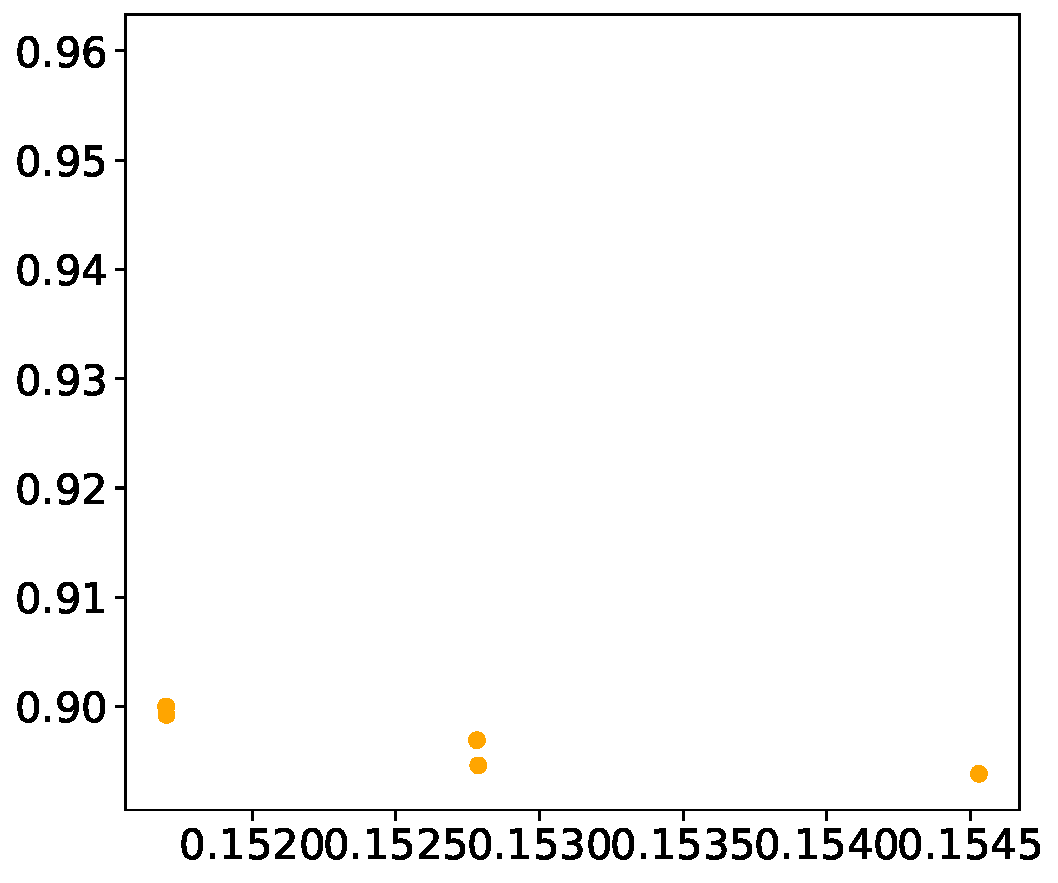
\includegraphics[width=\linewidth]{fig_GPR_RBF.pdf}
    \put(-200,85){$f_\text{tc}$}
    \put(-100,-5){$f_\text{cost}$}
\end{minipage}
\hfill
\begin{minipage}{0.48\linewidth}
    \centering
    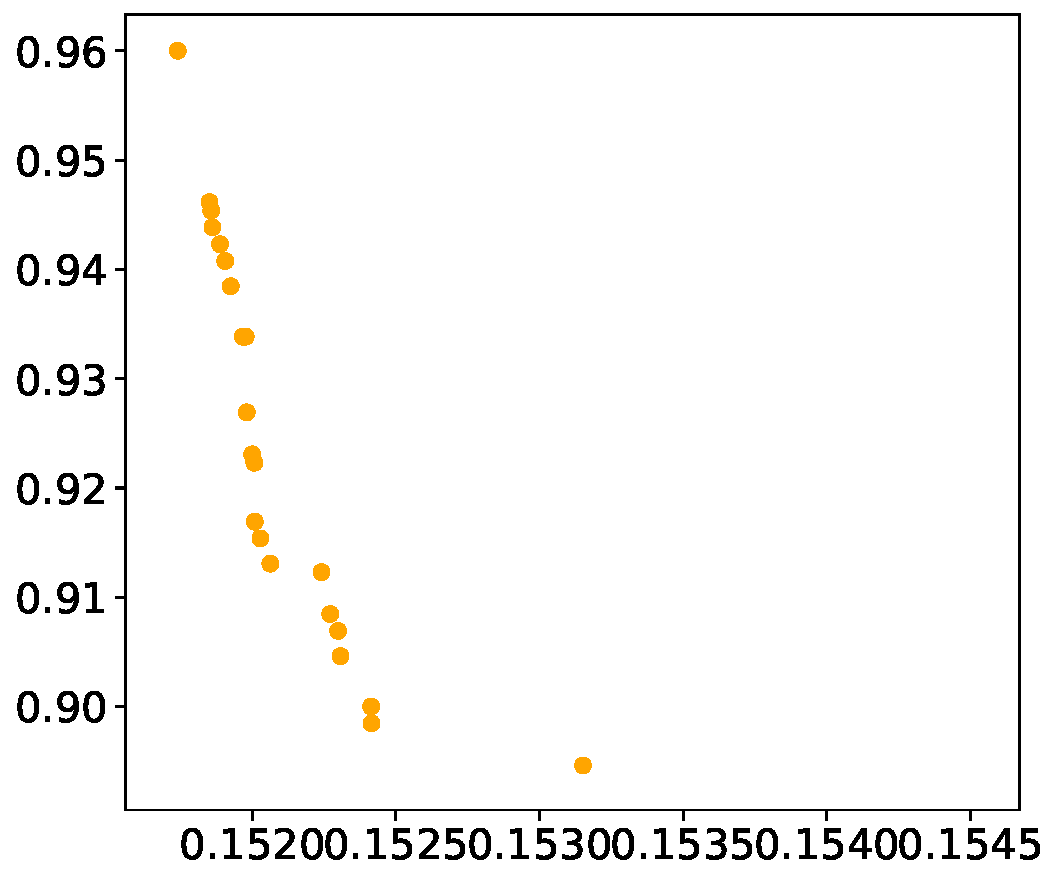
\includegraphics[width=\linewidth]{fig_GPR_RBF_DR.pdf}
    \put(-90,-5){$f_\text{cost}$}
\end{minipage}
\caption{Objective values of nondominated solutions obtained by GPR (RBF) and NSGA-II. Left: Standard method. Right: Dual-ranking variant.}
\label{fig:gpr_rbf_nd}
\end{figure*}


% Figure 2: GPR (Mat\'ern)
\begin{figure*}[htbp]
\centering
\begin{minipage}{0.48\linewidth}
    \centering
    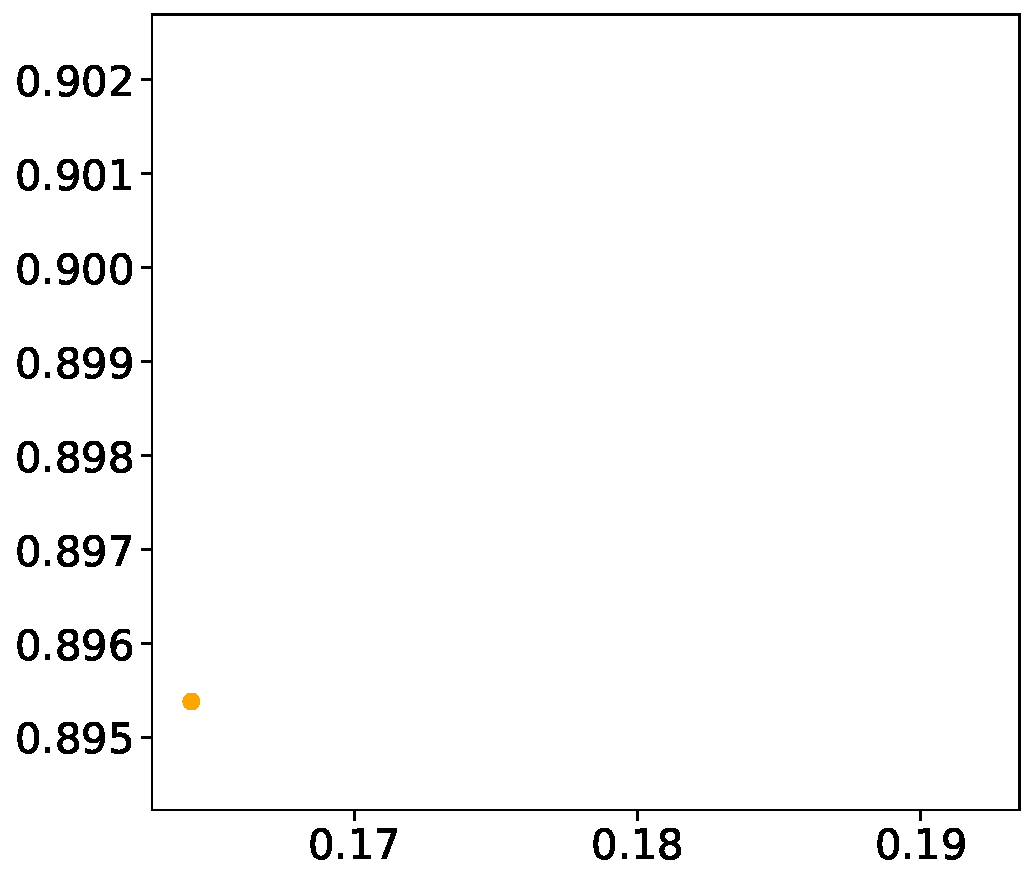
\includegraphics[width=\linewidth]{fig_GPR_Matern.pdf}
    \put(-200,87){$f_\text{tc}$}
    \put(-100,-5){$f_\text{cost}$}
\end{minipage}
\hfill
\begin{minipage}{0.48\linewidth}
    \centering
    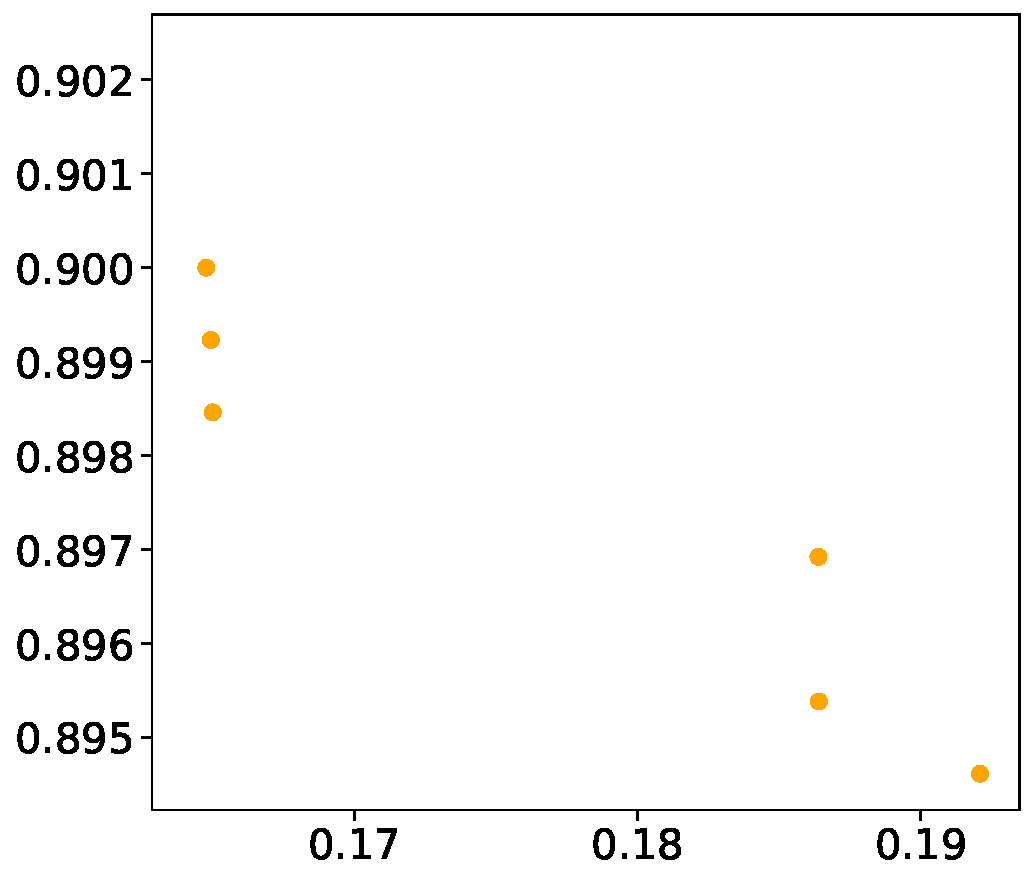
\includegraphics[width=\linewidth]{fig_GPR_Matern_DR.pdf}
    \put(-90,-5){$f_\text{cost}$}
\end{minipage}
\caption{Objective values of nondominated solutions obtained by GPR (Mat\'ern) and NSGA-II. Left: Standard method. Right: Dual-ranking variant.}
\label{fig:gpr_matern_nd}
\end{figure*}


% Figure 3: Autogluon-QR
\begin{figure*}[htbp]
\centering
\begin{minipage}{0.48\linewidth}
    \centering
    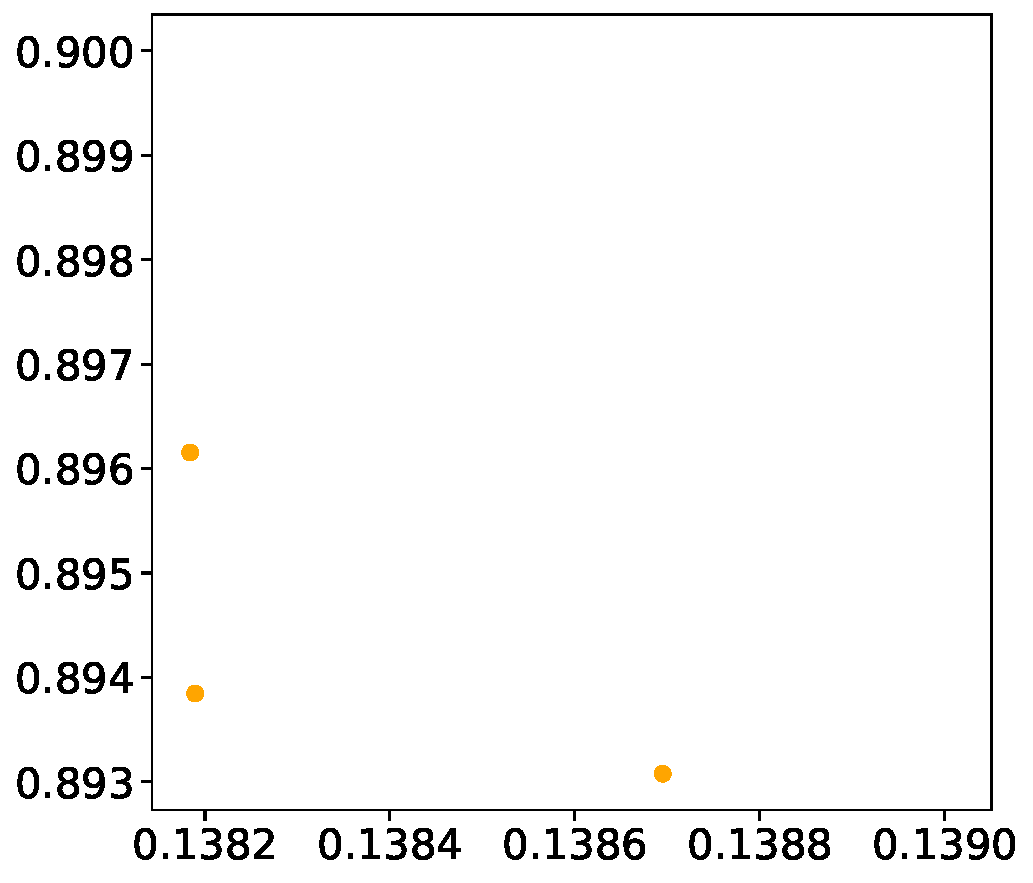
\includegraphics[width=\linewidth]{fig_QR.pdf}
    \put(-200,87){$f_\text{tc}$}
    \put(-100,-5){$f_\text{cost}$}
\end{minipage}
\hfill
\begin{minipage}{0.48\linewidth}
    \centering
    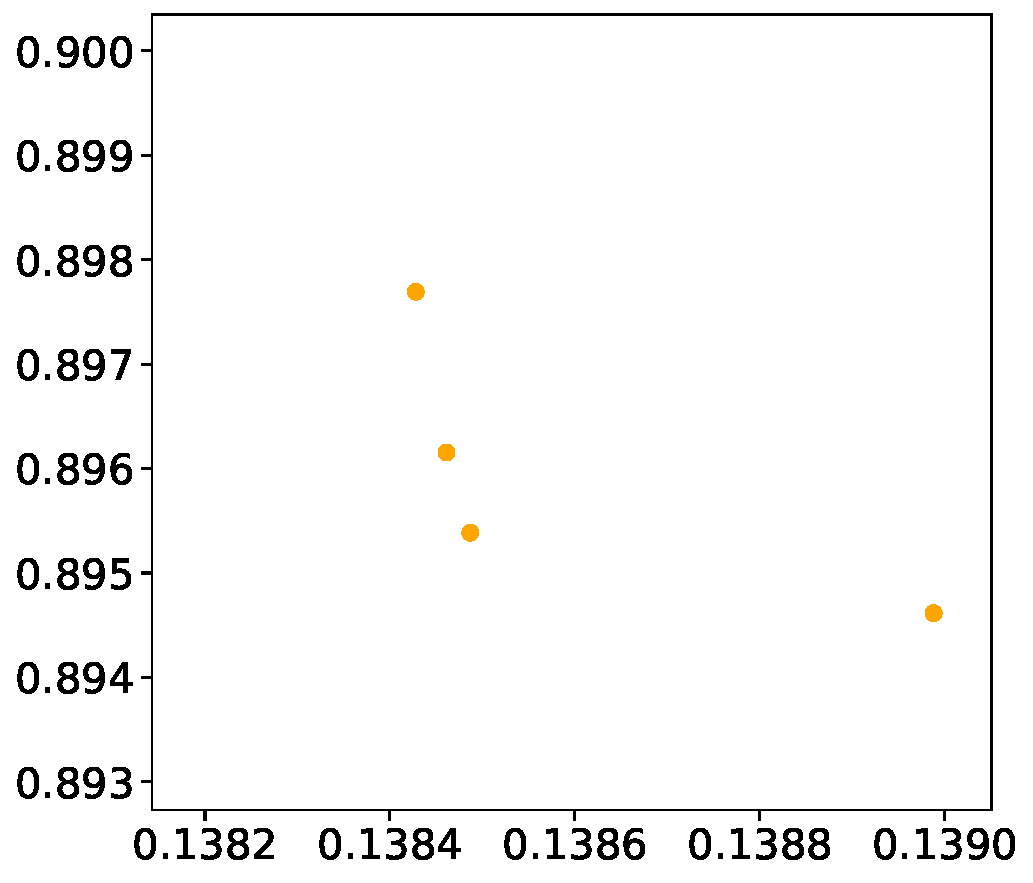
\includegraphics[width=\linewidth]{fig_QR_DR.pdf}
    \put(-90,-5){$f_\text{cost}$}
\end{minipage}
\caption{Objective values of nondominated solutions obtained by QR and NSGA-II. Left: Standard method. Right: Dual-ranking variant.}
\label{fig:qr_nd}
\end{figure*}


% Figure 4: BNN
\begin{figure*}[htbp]
\centering
\begin{minipage}{0.48\linewidth}
    \centering
    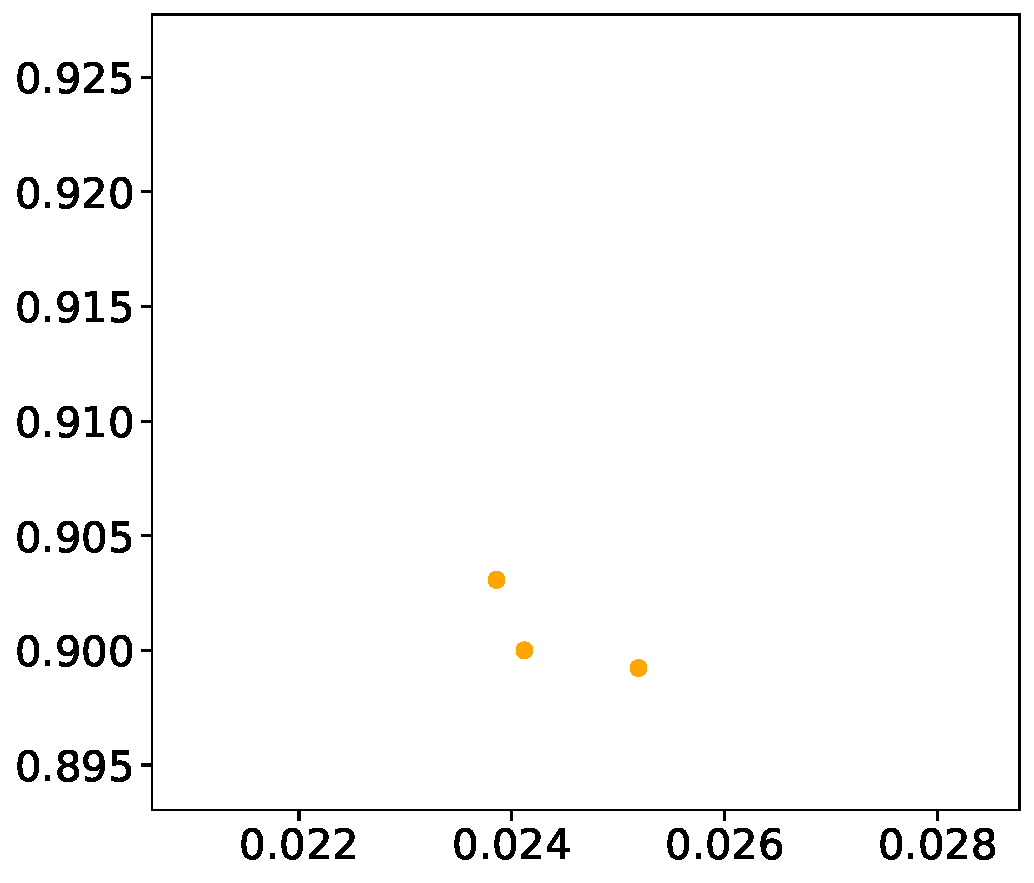
\includegraphics[width=\linewidth]{fig_BNN.pdf}
    \put(-200,87){$f_\text{tc}$}
    \put(-100,-5){$f_\text{cost}$}
\end{minipage}
\hfill
\begin{minipage}{0.48\linewidth}
    \centering
    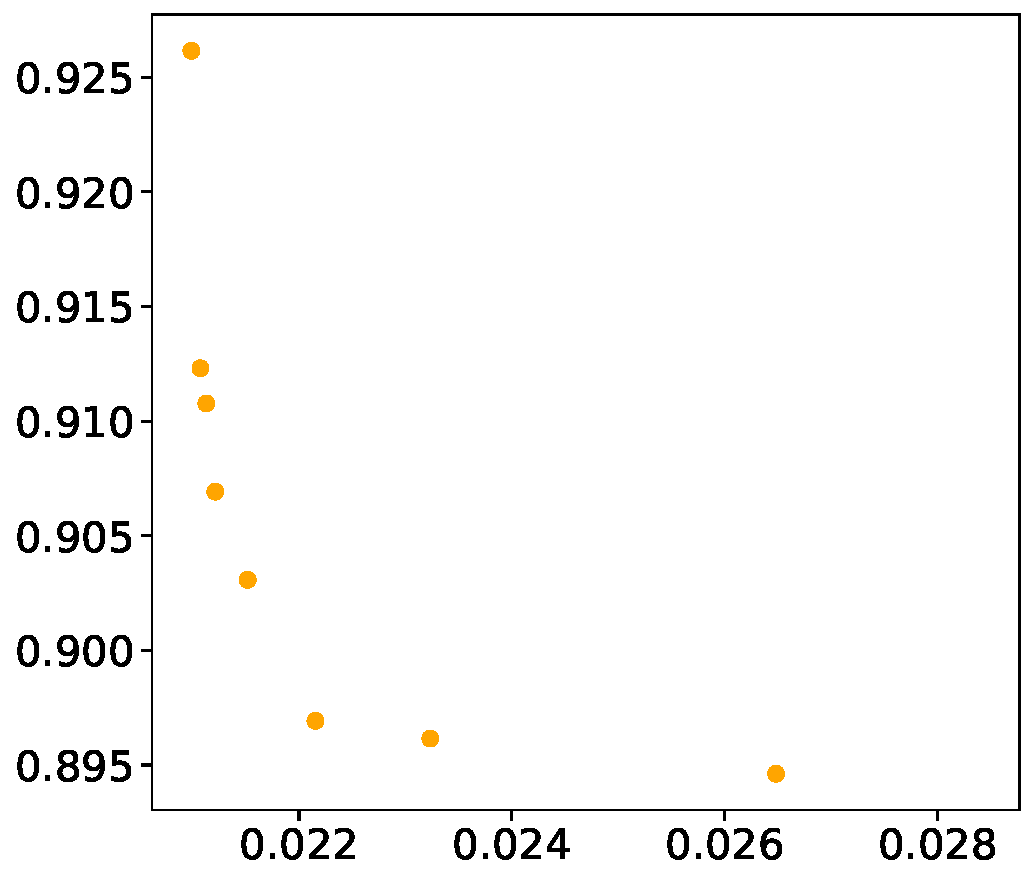
\includegraphics[width=\linewidth]{fig_BNN_DR.pdf}
    \put(-90,-5){$f_\text{cost}$}
\end{minipage}
\caption{Objective values of nondominated solutions obtained by BNN and NSGA-II. Left: Standard method. Right: Dual-ranking variant.}
\label{fig:bnn_nd}
\end{figure*}

\begin{table*}[htbp]
\centering
\caption{Comparison of the average number of obtained solutions between standard and dual-ranking variants.}
\label{tab:num_solutions}
\begin{tabular}{lcc}
\hline
Methods & Standard & Dual-ranking variants \\
\hline
GPR (RBF)    & 11.6 & 97.2 \\
GPR (Mat\'ern) & 3.4  & 36.2 \\
QR     & 3.4  & 11.6 \\
BNN    & 6.4  & 25.0 \\
\hline
\end{tabular}
\end{table*}

\newpage
\input{checklist.tex}


\end{document}